\documentclass[UKenglish, a4paper]{ifimaster}
\usepackage[latin1]{inputenc}
\usepackage[T1]{fontenc,url}
\urlstyle{sf}
\usepackage{babel,textcomp,csquotes,ifimasterforside,varioref,graphicx}
\usepackage[backend=biber,style=numeric-comp]{biblatex}
\usepackage{pifont}
\usepackage{booktabs}
\usepackage{verbatim}
\usepackage{listings}

\lstset{%
    captionpos=b,
    tabsize=2,
    breaklines=true
}

\newcommand{\cmark}{\ding{51}}
\newcommand{\xmark}{\ding{55}}
\newcommand{\ampers}{\&}
\newcommand{\demo}{VizPub}

\title{Visualizing and Evaluating the Performance of Overlay-Based Pub/Sub Systems}
\subtitle{}
\author{Nils Peder Korsveien}

\addbibresource{bibliography.bib}

\begin{document}
\ififorside{}
\frontmatter{}
\maketitle{}

\chapter*{Abstract}
\tableofcontents{}
\listoffigures{}
\listoftables{}
\chapter*{Aknowledgements}
\mainmatter{}

\chapter{Introduction}
\section{Thesis Outline}

\section{Motivation}

The publish/subscribe communication paradigm is receiving an increasing
amount of attention from the research community, as it provides a
loosely coupled and scalable interaction scheme suitable for large-scale
distributed systems~\cite{Eugster:2003}. It has also shown to be a useful
approach for several business applications such as financial data
dissemination~\cite{tibcorv} and application integration~\cite{goops}.
Topic-based pub/sub has also seen more novel applications such as
decentralised social networks. More specifically, the issue of
delivering notifications in such a network is a task especially suited
for this approach. This motivates further investigation into such
systems, comparing their performance and analysing their
characteristics and shortcomings.

\section{Problem Statement}


\chapter{Background}
\label{ch:background}
\section{The Peer-to-Peer Network Architecture}
In the peer-to-peer network architecture, every node in the network
contributes with its resources, including both storage space and
processing power.

%TODO read xl survey introduction for a good description

\section{The Publish-Subscribe Communication Paradigm}

Publish-Subscribe is a fully asynchronous, loosely coupled,
highly scalable, event-based messaging pattern. There are three main
system components in the pub/sub interaction scheme: the publishers, the
subscribers and the event service. The publishers publish events, and
the subscribers subscribe for events, while the event service handles
managing both subscriptions and publications, as well as routing events
to the subscribers. The basic architecture of a typical pub/sub system
is outlined in Figure~\ref{fig:pubsubarch}.

\begin{figure}
\centering
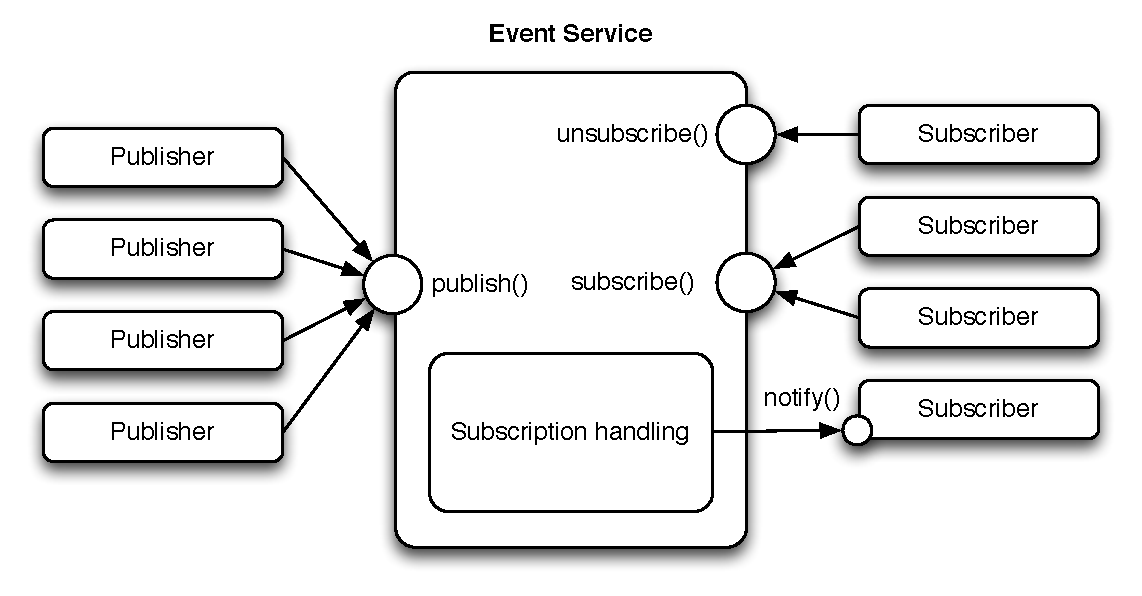
\includegraphics[width=\textwidth]{figures/pubsubarch}
\caption{The basic architecture of a pub/sub system.}
\label{fig:pubsubarch}
\end{figure}

The event service functions as an intermediary between publishers and
subscribers. It provides a level of indirection, as well as an service
interface. Publishers are able to generate new events through the
\texttt{publish} service call. It is now the responsibility of the event
service to determine which subscribers are interested in receiving this
event, and how to route the event to them. The subscribers register
their interest through a \texttt{subscribe} service call. The event
service will then store each subscribers interest in order to
disseminate events correctly. The publishers are then able to cancel
their subscriptions through a \texttt{unsubscribe} service call. No
information is forwarded from subscribers to publishers or from
publishers to subscribers.

The pub/sub paradigm provides a higher degree of decoupling than other
traditional approaches. In general there are three types of decoupling
pub/sub system provides us with:

\begin{description}
  \item[Space decoupling] The publishers and subscribers does not need to
    know about each other.
  \item[Time decoupling] Events are delivered regardless of whether or
    not publishers and subscribers are online at the same time.
  \item[Synchronization decoupling] Neither publishers nor subscribers
    are blocked when attempting to perform their operations.
\end{description}

While many other approaches can provide the first two forms of
decoupling, the main advantage of pub/sub is its fully asynchronous nature.
Approaches such as tuple spaces or message queues cannot completely
provide this synchronous decoupling, as messages are retrieved in a
synchronous manner. This property is key to the suitability for pub/sub
in large distributed system.~\cite{Eugster:2003}

\subsection{Message Filtering in Pub/Sub}

The subscription semantics of the pub/sub paradigm plays an important
role in the performance and flexibility of the system as event messages
are routed and managed based on topic or content. There are three
distinct types of subscription schemes:

\begin{description}
  \item[Topic-based] Events are split into topics, usually represented by
      a string.
  \item[Type-based] Filters events based on the structure of the data.
      Provides type safety at compile time.
  \item[Content-based] Events are filtered based on a global
      list of universal event attributes.
\end{description}

Content-based provides better expressiveness in terms of filtering out
the relevant events. However, this comes at the cost of higher overhead
with regards to handling subscriptions. The complex filtering algorithms
limit the scalability of such systems with regards to the number of
subscriptions. Type based is similar to content-based in the sense that
the public members of the types together form a description of the
content of the event. Although this ties the implementation of the
pub/sub system closer to the programming language, it still suffers from
the same drawbacks as content-based.

Topic-based offer less expressiveness than the other two subscription
schemes, but better performance if the set of possible event properties
is limited. Also, topic-based is more suited for dissemination and
multicasting, as topics can be thought of as groups, where subscribing
to topic T can be equivalent to joining the group for that topic. This
is a common approach taken by several proposed pub/sub
systems\cite{needs citation}.

Traditionally, reliable multicasting of data through deterministic
dissemination has been the common approach. However, more recent
implementations investigate the potentials of probabilistic protocols,
which are more suited to the nature of decentralized systems and P2P.
These protocols do not guarantee full reliability, but provides a high
quantifiable \emph{probability} that events are delivered to all
subscribers.

\section{Overlays}

\section{The Gephi Open Graph Viz Platform}

\begin{figure}
    \centering
    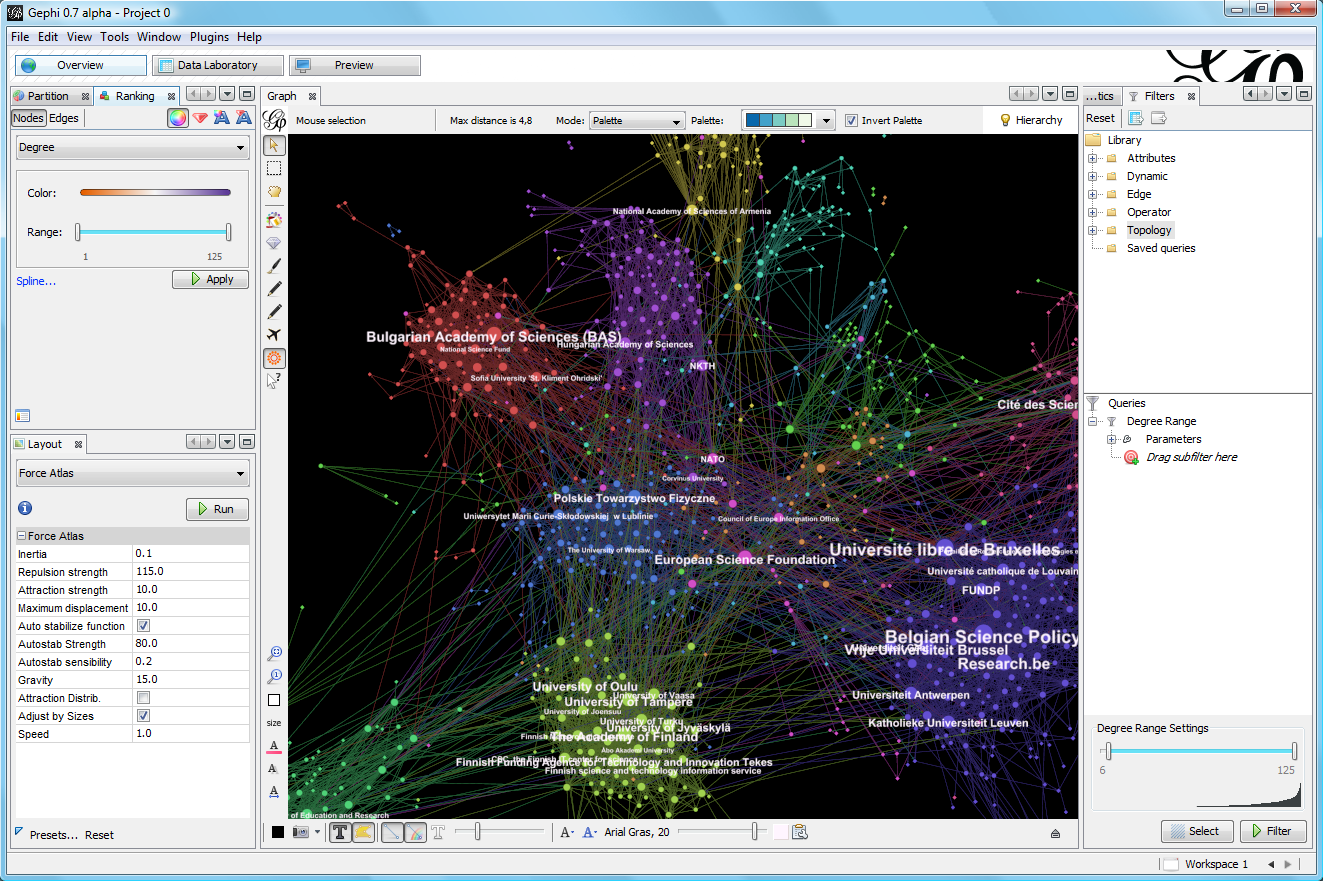
\includegraphics[width=\textwidth]{img/gephi1}
    \caption{The Gephi Tool supports
        visualization of graphs through coloring and sizing the visual
        graph
        representation. It also enables adding labels to nodes and
        edges. In
        this screenshot, Gephi is used to detect and visualize
    communities.}
\label{img:gephi1}
\end{figure}

Gephi~\cite{ICWSM09154} is an open source tool for exploring and
visualizing all kinds of networks, including dynamic and hierarchical
graphs. Described by the authors as ``photoshop for graphs'', Gephi
enables the user to interact with the graph structure, as well as
manipulate the colors and sizes of the visual graph representation in
order to display graph properties in an intuitive way. Gephi aims to
help researchers and data analysts in discovering patterns and revealing
hidden properties of the graph in question, as well as easily
discovering errors in the dataset. Gephi also provides a set of
statistical tools for measuring common metrics for Social Network
Analysis~(SNA) such as centrality, as well as metrics useful for general
graph topology analysis such as degree, path length and clustering
coefficient. Gephi is also useful in the emerging field of Dynamic
Network Analysis~(DNA)  as it supports temporal graphs, giving the user
the ability to filter the graph model according to a defined time
interval. It also support playback of the graph evolution, as well as
visualizing changes to graph data over time through size, color and text
labels which can be applied to both nodes and edges.

Gephi provides a rich GUI-experience where users may interact with the
graph representation, apply layout algorithms, filter the graph
representation, execute metrics, apply color and size based on graph
properties and animate the graph evolving over time through the timeline
component. The Gephi software architecture is highly modular and
supports extensions via plugins, some of which are available in a
official plugin marketplace found at~\cite{gephimarketplace}. New
metrics, filters or database support may be implemented through such
plugins by developers and published to the marketplace free of charge.

Gephi provides many tools and components which are useful in the context
of researching and analysing pub/sub overlays.

\subsection{Useful functionality in Gephi}

\begin{description}

\item[Node and Edge pencil tools] \hfill \\

    These two tools enable the user to create nodes and edges by
    clicking in the graph view. Edges can be undirected or directed,
    where direction is indicated with an arrow. These two tools combined
    enables building a graph by hand.

    Building such graphs can be useful in order to reason, analyse or
    learn network algorithms, such as event dissemination algorithms. In
    this case, the user can start with a single node which can act as
    the event source, and build the topology as the event disseminates,
    carefully following the particular algorithm in question when doing
    so. The user can also add attributes to the nodes and edges either
    through the node query tool or in the Data Laboratory component
    which also aids in visualising and understanding properties,
    drawbacks and advantages of such algorithms.

\item[Node Query Tool] \hfill \\

    With the node query tool the user is able to click on a node on the
    graph model, and a panel which will display a panel with information
    regarding the properties and attributes of this node. Properties include
    data describing the visual properties of the node such as size, position
    and color. Attributes include the Id and Label and Time Interval
    attributes and any additional user defined attributes. In our case, such
    user defined attributes would include Topics, Subscription Size and
    Gossips Sent/Received.

    Both the properties and attributes of the node are editable through this
    panel view. The user can select a property to change the visual
    representation of the node, or the attributes to change their value. The
    Time Interval attribute is interesting to edit in particular as it
    represents the points in time in which a node exists in the graph model.
    On example scenario is editing the Time Interval attribute for a certain
    nodes in order to see how it affects a particular metric as well as the
    overlay topology.

\item[Shortest Path Tool] \hfill \\

    With the Shortest Path Tool selected, the user may click on two nodes on
    the graph model, and if there is a shortest path between them, this path
    will be highlighted with a color. It might be useful to reason about the
    relationship between key nodes in the graph, or to compare shortest path
    between several pairs of nodes. (more use cases?)

\item[Heat Map Tool] \hfill \\

    The heat map tool enables the user to click on a node in the graph model
    and color its neighborhood based on the edge weight distance between
    them. More specifically, it sets the node color intensity lower for more
    distant nodes and stronger for nodes that are closer. Edge weight is a
    standard edge attribute that are by default set to 1. This means that in
    the default case, the visualization will represent the hop count
    distance from the particular node selected by the user. However, the
    edge weight can be edited by the user in order to represent other
    properties of a system. As an example, imagine setting the edge weight
    to represent network latency between two nodes. In this case, a
    neighboring node which is adjacent to the selected node would have a
    lower color intensity if the latency between them is higher than another
    neighboring node which is further away in terms of hop count.

\item[Timeline Component] \hfill \\

    The timeline component introduces an animation scheme for dynamic
    graphs. The user may choose playback parameters such as time
    interval size, step size and playback speed. The time interval will
    filter out a subgraph defined by the upper and lower bound of the
    interval. The evolution of the dynamic graph will then be animated
    by moving these bounds by the distance defined by the step
    parameter. The delay between each step is decided by the playback
    speed.

    The timeline enables the user to visually inspect the change in
    graph topology over time, as well as visualize and inspect node and
    edge attributes of the graph through both color, size and text
    labels which is able to change dynamically as part of the graph
    model animation. The timeline also enables jumping to a specific
    point in time and investigating the corresponding subgraph and its
    properties by changing the upper and lower bound of the Time
    Interval.

\item[Statistics Component] \hfill \\

    The metric component enables graph topology analysis by executing
    metrics on the graph. There are two types of metric algorithms in Gephi:
    static and dynamic. Static metrics are only able to execute on graph
    model representing a single point in time, while dynamic will traverse
    the time line by executing the metric iteratively across a set of time
    intervals. When executing a dynamic metric, the user is able to choose
    window size and time step. The window size is a time interval which will
    be moved by the step size defined by the user. Metrics are divided
    into \emph{static} and \emph{dynamic} metrics, where the former
    calculates a single value based on the currently defined time
    window, while the latter calculates a time series of values. When
    executing a dynamic metric, the user must define the time window
    size, and tick. The have the same functionality as step parameter
    when using the \emph{Timeline Component}. When the metric executes,
    the time window will iterate through the entire time range of the
    simulation, calculating a static metric at each step. When finished,
    a time series is plotted and displayed for the user.

    The Statistics component include several metrics which are relevant
    to pub/sub overlays. Useful static metrics include, but are not
    limited to:

    \begin{itemize}
        \item{Degree (In/Out/Avg./Max/Min/Distr.)}
        \item{Avg. Cluster Coefficient}
        \item{Centrality (Beetweeness/Closeness/Eccentricity)}
        \item{Average Path length}
        \item{Radius}
        \item{Network Diameter}
        \item{Number of Shortest Paths}
    \end{itemize}

    Of these, only degree and the clustering coefficient metrics have dynamic
    versions, where both calculates the average value over time. The
    average for dynamic metrics are calculated by dividing the sum of
    all node attribute values with the total number of nodes in both
    cases.

    %TODO: describe exactly what sort of averages/data are calculated by
    each metric

\item[Ranking Component] \hfill \\

    The ranking component is a key feature of Gephi which enables
    visualization based on node or edge attributes in form of color
    and size. When coloring nodes or edges, the ranking component
    will apply a gradient over the range of attribute values. The
    ranking component also include a Result list, where the user may
    sort nodes based on the specified attribute value, which is
    useful for quickly finding the nodes with maximum value and
    minimum value, which might help in identifying bottlenecks in
    the system or potential load balancing issues.

    The Ranking component also includes an Auto Apply feature, which
    supports vizualising attributes dynamically while playing back the
    graph via the Timeline Component.

\item[Layout Component] \hfill \\

    The Layout component enables the user to execute algorithms that
    calculates the position of the nodes. The user is able to adjust the
    parameters of these algorithms in order to manipulate the visual
    layout. The different algorithms emphasize different aspects of the
    topology. One example is the Force Atlas layout algortihm which
    simulates the effect of gravity on the nodes where linked nodes
    attract each other, and non-linked nodes are pushed apart. This
    particular algorithm is useful for visually detect clusters and
    communities. Another useful algorithm is the Circular Layout
    algorithm, where nodes are positioned in a circle ordered on a
    specific attributes selectable by the user. This is useful in order
    to visualize node rankings on particular attributes.

\item[Filter Component] \hfill \\

    Filter may be applied to the graph in order to strip away nodes or
    edges on the basis of their attributes which also includes any
    calculated metrics. Filters may strip away based on a value range if
    the attribute type is a number, or a regex match if the attribute is
    a string. Filters can be combined through special operator filters
    representing set operations such as union and intersect.

    Filters are an essential mechanism in order to analyze subgraphs.
    One use example is the case of calculating topic diameters in pub/sub systems,
    where a subgraph can be filtered on a topic attribute. This
    allows executing the diameter metric on the resulting subgraph
    on the selected topic.

\item[Data Laboratory Component] \hfill \\

    The Data laboratory component enables the user to work with the node
    and edge attributes of the graph. This component provides the user
    with separate table views of node and edge attributes. Each row in
    these table represent a node or edge, and columns may be added or
    removed by the user. The Data Laboratory also provides functionality
    for manipulating columns such as merging two columns or creating new
    columns based on data from the existing columns. Attribute data
    in columns that are static (i.e.\ has no lower or upper time
    interval bound associated with them) can be converted to dynamic
    through this component. Also, resizing or coloring all edges or
    nodes is possible through the laboratory by selecting all rows
    and right-clicking.

    The laboratory also enables the user to export the data to file
    for further statistical analysis.
\end{description}


We consider tools such as Gephi to be a valuable addition to the field
of P2P protocol research. Visual Exploration of a dynamic network graph
is a useful approach to evaluating these protocols, as some properties
of the system are more easily spotted visually. For example, during our
implementation work, it was trivial to visually confirm that some edges
were missing from the graph, leading to the discovery of a critical bug
in the implementation code which would otherwise be difficult to spot.
It is also worth to note that the different actors involved in the Gephi
project has formed a legal entity in the form of The Gephi
Consortium~\cite{gephi-consortium} in order to assure future development
of this tool. This provides us with a certain degree of assurance that
this project is something well worth investing in, as the risk of it
being discontinued seems unlikely at this point in time.

\section{The Gephi Toolkit}

In addition to the GUI-client, the authors of Gephi also provide an API
through the Gephi Toolkit project. The toolkit packages essential
modules from the GUI-client into a standard Java library which can
be used by any stand-alone Java project by including it as a dependency.
We take advantage of this toolkit in our implementation work, where it
is mainly used to handle and store reports collected from PeerNet
simulations.

\section{The GEXF File format}

The GEXF (Graph Exchange XML Format) file format~\cite{gexf} is an
effort by the Gephi Consortium to define a standard language describing
complex network structures. Being developed by the same group of people,
the Gephi Tool is naturally fully compatible with this format, and is
able to both import and export GEXF files. This is also the case with
the Gephi Toolkit, as the module for handling such imports and exports
are included in this toolkit as well.

The GEXF file format is able to describe a graph through its nodes and
edges, as well as any data and dynamics associated with the graph. More
specifically, the file format is able to describe node, edges and their
associated attributes. Listing~\ref{lst:gexf-basic} provides an example
of a minimal static GEXF file, describing nodes, edges and attributes of
a graph.

\begin{figure}
\lstinputlisting[language=XML, label=lst:gexf-basic, frame=single]{listings/basic.gexf}
\caption{A GEXF description of a minimal static graph}
\end{figure}

\subsection{Dynamics}

One of the major advantages of this file format is its support for
dynamic functionalities.  Both nodes, edges and attributes may have a
defined time interval where they exist. These lifetime intervals are
described as ``spells'' if applied to nodes and edges, and as ``start''
and ``end'' XML-attributes if applied to node or edge attributes. The
GEXF file in Listing~\ref{lst:gexf-dynamics} shows an example of a
dynamic graph where spells are used in order to determine the lifetime
of the nodes.  The start and end times are by default encoded as
doubles, however, dates are also supported, as seen in this example.

The
support for dynamic graphs makes this file format an interesting option
for storing simulation data, and in our implementation work we use this
format extensively as part of our research effort.

\begin{figure}
\lstinputlisting[language=XML, caption={}, label=lst:gexf-dynamics,
frame=single] {listings/dynamics.gexf}
\caption{Example of  dynamic GEXF file using spells}
\end{figure}

\section{The PeerNet Simulator}

\subsection{Event Engine}

\subsection{Protocols}

\subsection{Observers}



\chapter{Design Challenges in Topic-Based Pub/Sub}
% Provide a mini survey of existing pub/sub system. Might have to go
% through some rewrites.
\label{ch:design-challenges}
Designing decentralized topic-based pub/sub systems is a big research
challenge due to a number of desired system properties which are in
conflict with eachother. For example, making the
overlay robust is difficult without introducing too many redundant edges
in the network graph.  Many approaches to topic-based pub/sub have been
proposed the last
decade~\cites{Baehni:2004}{Castro:2002}{Chockler:2007}{Rahimian:2011}{Girdzijauskas:2010}{Matos:2010}{Wong:2008}{Zhuang:2001}.
And each have made trade-offs in an attempt to balance the system
properties against each other. In this chapter, we extend the
mini-survey found in~\cite{Setty:2012}, were we include a number of
additional protocols. Also, we will go more into detail regarding the
design challenges found in topic-based pub/sub system by illustrating
the charachteristics of these systems, as well as their shortcomings.

\section{Desired System Properties}

In order to provide correct and efficient delivery of notifications in a
decentralized OSN using topic-based pub/sub, a high number of system
properties are deemed desirable~\cite{Setty:2012}. More specifically,
these challenges include:

\begin{description}

    \item[Correct delivery]\hfill\\
        All notifications should be delivered to the
        correct recipient. Both false positives and false negatives should be
        avoided.

    \item[High hit-ratio during churn]\hfill\\
        Notifications are delivered to a very high
        percentage of subscribers in the presence of churn. In the
        absence of churn, notifications should be delivered to all
        subscribers. This is similar to correct delivery except for
        not taking false positives into account.

    \item[Fast recovery]\hfill\\
        The overlay should quickly recover from a
        period of churn. Nodes should be able to both leave and join the
        network gracefully, and nodes who are dead should be properly
        handled by the system.

    \item[Low average node degree]\hfill\\
        The overlay nodes should have a low
        node degree as possible to achieve scalability with regards to number of
        topics. The degree distribution should be as even as possible,
        in order to achieve load balancing.

    \item[Topic connectivity]\hfill\\
        The routing of an event only includes the
        subscribers who registered their interest for the topic. This is
        also known as \emph{relay-free routing}.

    \item[Scalability]\hfill\\
        The system should scale in terms of number of
        topics, number of nodes, number of topics a node is interested in and
        number of nodes interested in a topic.

    \item[Efficient dissemination]\hfill\\
        Event dissemination should have a low
        delay with little duplicate delivery, and the load of routing messages
        should be distributed fairly.

    \item[Low overlay maintenance cost]\hfill\\
        Managing the overlay topology
        should be as inexpensive as possible. Maintenance might include mending
        dissemination structures such as multicast trees when nodes fail, but
        also how to include joining nodes in the structure and allowing nodes to
        leave gracefully.

\end{description}

Designing a system with all of these properties
presents a challenge, as several of the desired characteristics are
fundamentally at odds with each other. Maintaining a low node degree
makes it difficult to maintain \emph{topic connectivity}, while
avoiding duplicate message delivery conflicts with being robust in the
presence of churn. There is also a trade-off in robustness and
reliability depending on the approach taken to disseminating messages.
Specialized overlays that build dissemination structures such as
multicast trees provide fast and reliable message delivery with no
duplication of messages. However, they are fragile and susceptible to
churn. Epidemic dissemination on the other hand is more robust, but does
not provide full reliability as it lacks deterministic delivery
guarantees.

There is also a trade-off between the navigability of the overlay and
the message overhead. Stanley Milgram famously demonstrated the
\emph{small-world phenomena} in~\cite{milgram1967small} where he showed
that any two participants in a network was likely to be connected
through a low number of intermediaries. Taking this phenomena into
consideration has proved to be a useful approach when constructing
decentralised overlays, as they provide a highly navigable network due
to the small average shortest path length. A popular approach is to
create one or more long jump links between nodes to provide better
routing capabilities. More specifically, these links are usually created
by utilizing a distance function in the name space, where the
probability of creating a link increases with the distance between them.
The subscription interest of such nodes are usually not taken into
consideration when creating such links. Consequently, the message
overhead in the system is increased as more relays are introduced in the
overlay.

Many existing systems suffer from shortcomings that originate from wanting
to include a high number of desired properties described above. This
motivates further research into these systems and how they compare in
terms of promoting these desirable properties.

\section{Handling Trade-offs}

Designers of existing approaches have been facing the challenges of
handling the trade-offs discussed in the previous section. One of these
challenges is building both a reliable and robust overlay. A naive
approach to this problem would be to create a separate overlay for each
topic as in TERA~\cite{Baldoni:2007}. However, this approach suffers from
poor scalability as the number of nodes and topics increase. Another
approach would be to structure the overlay by creating a spanning tree
per topic as seen in Scribe~\cite{Castro:2002}, Bayeux~\cite{Zhuang:2001}
and Magnet~\cite{Girdzijauskas:2010}. However, these structures are
conceptually fragile in the presence of churn, requiring mechanisms for
mending the structure when nodes fail. This increases the overhead of overlay
maintenance.  Also, the root node of the spanning tree represents a
single point of failure as well as a bottleneck in the system. This is
especially true for popular topics where all events must travel through
the root node. In Scribe, the root node is used as a \emph{rendezvous}
point for topics by using the routing capabilities of the underlying
Pastry DHT~\cite{Rowstron:2001}. Such dedicated nodes represent a
single point of failure in addition to being detrimental to load
balancing and scalability.

Minimizing the average node degree while simultaneously achieving a
\emph{topic-connected overlay} (TCO) is another difficult trade-off to
consider. Topic-connectivity is achieved when no other than the
nodes who registered their interest in a topic takes part in routing
events for that topic. The desired goal with regards to
topic-connectivity is not only to avoid routing events through
uninterested nodes, but also to minimize the node degree by reusing
links for several topics. This approach achieves better scalability with
regards to the number of topics in the system.  Also, it decreases the
message overhead incurred by both event dissemination and overlay
maintenance mechanisms such as heartbeat messages. In addition to this,
keeping an overlay topic-connected simplifies the message routing
mechanism as no designated relay or gateway node needs to be implemented
in the protocol such as in Scribe and Vitis.

ElastO~\cite{Chen:2013} propose an interesting approach to overlay
construction, where the goal is to construct a TCO while maintaining a low
node degree. The construction of the overlay is performed by a
centralized component which requires global knowledge, while the
maintenance of the overlay is performed in a distributed manner in
response to churn events. By using a centralized algorithm for overlay
construction, ElastO is able to provide a more optimal TCO than decentralized
solutions, while still maintaining the high performance of a
decentralized repair mechanism to handle node departure or arrival.

With regards to the reuse of links for several topics, an observed
correlation~\cite{Liu:2005} between subscription sets in practical
workloads is useful to consider when constructing overlays. This
observation is exploited in Poldercast in order to decrease the number of
links to maintain. Also, it is used as a basis for overlay construction
in both StaN~\cite{Matos:2010} and SpiderCast~\cite{Chockler:2007}.
However, these two protocols only provide a probabilistic guarantee that
the resulting overlay will be fully topic-connected. In contrast,
PolderCast claim deterministic guarantees of providing a TCO. However,
this relies on two factors: (1) that there is no churn in the system,
and (2) that the underlying Cyclon~\cite{Voulgaris:2005} protocol, which
is used for peer sampling in PolderCast, can guarantee a connected
overlay.  Consequently, the deterministic guarantees of PolderCast could
be questioned.\ daMulticast~\cite{Baehni:2004} on the other hand provide
a deterministic guarantee of topic-connectivity through quite a
different approach of overlay construction. More specifically,
daMulticast constructs a topic hierarchy, where events are disseminated
through gossiping each level of this hierarchy in a bottom-up approach.

As mentioned in section 2, several protocols attempts to create an overlay that
exhibits \emph{small-world properties}. In Vitis, the subcluster
together with the relay paths form an overlay similar to a small-world
networks, which decreases the routing delay, but includes
uninterested gateway and relay nodes. In Magnet, small-world properties
are provided by the underlying Oscar DHT~\cite{girdzijauskas2007oscar}
which cluster similar nodes together.

\subsection{Overlay construction}

There are several different approaches to overlay construction.
Structured approaches such as dissemination trees have already been
mentioned, but there are also unstructured approaches. In Quasar
\cite{Wong:2008}, a novel approach to event dissemination using random
walks removes the need for a structured overlay.  There are also hybrid
approaches to structuring overlays such as in ElastO~\cite{Chen:2013}
and Vitis~\cite{Rahimian:2011}. In ElastO, the bootstrapping of the
graph is performed by a centralized entity, while in Vitis nodes with
similar interests are clustered together. A topic in Vitis might consist
of several subclusters which are connected to each other through relay
paths. This creates an overlay that is similar to dissemination trees,
but where single nodes have been replaced with clusters of nodes.
However, the drawbacks are still similar to the ones found in systems
relying on multicast trees, as it relies on designated gateway nodes
within subclusters communicating with rendezvous nodes along the relay
path. In Poldercast~\cite{Setty:2012}, a structured ring per topic is
used in combination with a form of epidemic dissemination that resembles
gossiping. Publishers are themselves part of the ring of the topic they
publish, and the structures attempt to combined into themselves into a
single overlay through random links. Such an hybrid approach is an
attempt at balancing the reliability of a structured overlay with the
robustness of epidemic dissemination. When it comes to node degree
however, Poldercast might introduce hotspots in the system as the
distribution of random links might be skewed.

In Magnet, the aforementioned subscription correlation is used to build
dissemination trees such as the ones seen in Scribe and Bayeux. As
mentioned these structures are not ideal in dynamic systems as they
require maintenance. However, tree structures do have an advantage when
it comes communication overhead, as they in theory avoid any duplicate
messages. In practice however, duplicate messages might occur if a node
that is part of a tree is part of an underlying routing path to the root
node. For example, in Scribe, notifications are routed to the root node
of a topic tree using an underlying DHT. If a child node belonging to
this tree is part of the routing path, it will receive the same message
twice. Once while routing to the root, and once again from its parent
after the publication message has reached the root node. However, the
number of duplicates should still be lower than what is seen in systems
relying on epidemic dissemination schemes, such as daMulticast and
PolderCast. In such systems, the number of duplicate messages are indeed
higher, however, the increased number of control messages also has the
benefit of making these systems more resilient to churn. Furthermore,
there is usually an adjustable \emph{fanout parameter} in such systems
which can be manipulated in order to control the number of messages that
are forwarded by a node. Thus, there is some control over the amount of
communication overhead in these systems. Both PolderCast and daMulticast
include such a fanout parameter. Also, it bears mentioning that
structured overlays include communication overhead in the form of
structure maintenance and structure mending in the case of both node
failure as well as nodes leaving and joining the network. Control
messages such as heartbeats are commonplace in such protocols e.g.\ in
Scribe where the each non-leaf node in the multicast tree periodically
sends heartbeats to its children. This increases bandwidth consumption
and adds a higher communication overhead compared to unstructured
overlays where such maintenance usually is not required.

Node degree is another important issue to consider when designing
overlays. A low average node degree increases scalability as topics and
number of nodes in the system increases. In protocols who rely on an
underlying DHT, node degree is usually either constant or a logarithmic
function of the total number of nodes in the graph. Such is the case in
Bayeux which relies on the Tapestry DHT~\cite{tapestry}, or Scribe which
relies on the Pastry DTH~\cite{Rowstron:2001}. Other implementations
might have a constant node degree, which is the case in Vitis which
might result in the separation of a topic into subclusters. Some extreme
examples include TERA~\cite{Baldoni:2007} and
daMulticast~\cite{voulgaris:2007} which
has a node degree that grows in the order of the number of topics the
node has subscribed to.  In the worst case scenario, this is also the
case in PolderCast, as maintaining a low node degree depends on the
degree of correlation in the subscription sets.  Indeed, when using
workloads from Facebook, the node degree in PolderCast grows almost
linearly with subscription size, as shown in \cite{Setty:2012}. This
suggests a scalability issue in a scenario where the subscription
correlation is weak.

%{../tables/comp-overlay} <- vim gf
\begin{table}
\centering
\resizebox{\columnwidth}{!}{%
\begin{tabular}{ccccccc}
    \toprule
    Protocol                         & Overlay      & Structures? & TCO?\    & Central nodes* & sub.\ corr.? & Node degree \\
    \midrule
    Scribe~\cite{Castro:2002}        & Structured   & Trees       & \xmark{} & RV             & \xmark{}     & $O(\log|\mathcal{V}|)$ \\
    Magnet~\cite{Girdzijauskas:2010} & Structured   & Trees       & \xmark{} & Relays         & \cmark{}     & $O(1)$\\
    Bayeux~\cite{Zhuang:2001}        & Structured   & Trees       & \xmark{} & RV             & \xmark{}     & $O(\log|\mathcal{V}|)$\\
    Vitis~\cite{Rahimian:2011}       & Hybrid       & Trees       & \xmark{} & RV\ampers{}GW  & \xmark{}     & $O(1)$\\
    StaN~\cite{Matos:2010}           & Unstructured & None        & prob.    & None           & \cmark{}     & $O({|\mathcal{T}_v}|)$\\
    SpiderCast~\cite{Chockler:2007}  & Unstructured & None        & prob.    & WB             & \cmark{}     & $O(K\cdot(|\mathcal{T}_v|))$\\
    daMulticast~\cite{Baehni:2004}   & Unstructured & None        & det.     & None           & \xmark{}     & $\Theta({|\mathcal{T}_v}|)$\\
    Quasar~\cite{Wong:2008}          & Unstructured & None        & \xmark{} & None           & \xmark{}     & Unknown\\
    PolderCast~\cite{Setty:2012}     & Hybrid       & Rings       & det.     & None           & \cmark{}     & $O({|\mathcal{T}_v}|)$\\
    ElastO~\cite{Chen:2013}          & Structured   & Ring        & det.     & None           & \xmark{}     & $O({\rho \log |\mathcal{V}}| |\mathcal{T}|)$\\
    \bottomrule
    \multicolumn{5}{l}{*RV:\ Rendezvous GW:\ Gateway WB:\ Weak bridge}\\
\end{tabular}
}%
\caption{Comparison of the different protocols and their overlay properties}
\label{table:comp-overlay}
\end{table}


Table~\ref{table:comp-overlay} provides an overview over several
different state-of-the-art protocols, comparing their different system
properties such as topic connectivity and whether or not it takes
advantage of subscription correlation.  Note that
PolderCast has received the benefit of doubt in this table, and have
been marked as providing a deterministic guarantee of
topic-connectivity. Magnet has a different approach to the spanning tree
structures, where messages are disseminated bottom-up. This means that
the root node is not a rendezvous node according to  the traditional
definition~\cite{baldoni2005distributed}, but it is still conceptually
a single point of failure as it is responsible for propagating messages
back down the tree when it receives a message. In SpiderCast, there is a possibility
of the overlay forming into a pattern of highly connected clusters
inter-connected through a small number of links which we refer to as
\emph{weak bridges}. The node degree in SpiderCast also relies on the
\emph{K-coverage} parameter of the system, where, for each topic, a node
attempts to connect to $K$ neighbours who share the same interest.
Protocols who rely on a underlying DHT typically have a node degree
which grows logarithmically with the number of nodes in the system. The
exception is Magnet which leverages a DHT providing small-world
properties~\cite{girdzijauskas2007oscar}, creating a fixed node degree
that is independent of both subscription size and number of topics
\cite{Zhuang:2001}.  Note that the node degree in Quasar is omitted from
the table, as it is dependent on the implementation of the bloom filters
used to represent the neighbours. In ElastO, $\rho$ is a system parameter
which balances between average and maximum node degrees when choosing
new edges to recover from churn.

% Note that even though ElastO has a
% higher node degree than the centralized solutions, it provides a more
% optimal TCO.\

\section{Event dissemination}

In terms of event dissemination, it should be mentioned that some of
the systems described earlier do not concern themselves with this aspect, and
focus only on the construction and maintenance of the overlay
itself. More specifically, this includes SpiderCast, StaN and ElastO. Thus, any
discussion regarding dissemination technique or routing performance
will be irrelevant for these systems. For other systems however, a
comparison of techniques is in order.

As mentioned, the dissemination in systems relying on multicast trees
removes much of the message duplication and usually offers on average
dissemination of events in logarithmic time as is the case in Scribe,
Magnet and Bayeux. In Vitis, event dissemination is performed by
flooding inside the subcluster, while simultaneously forwarding the
event to other subclusters if needed. As mentioned, gossiping is the
main approach in both daMulticast and PolderCast.  Gossiping usually
implies an exponential dissemination speed, however, there might be
other implementation specific factors in play which inhibits this
property of gossiping. As an example, in PolderCast, skewed random link
distribution might be detrimental to the speed of the gossiping
protocol. The authors of Quasar~\cite{Wong:2008} propose quite a different approach
to event dissemination, as routing is performed by having nodes install
routing vectors in nearby overlay neighbours. Messages are disseminated
through random walks, which are directed towards the subscribers when
passing through a node with the relevant routing information. This
approach is likely to be highly robust against churn. However, as
observed in~\cite{Wong:2008} the hit ratio stagnates at 97\% in a
static system. This is due to a phenomenon where some group members
might be obscured by other members who absorb messages
from all directions. The authors suggest a solution by having node
periodically pull information from other nodes, but this introduces more
overhead in terms of network traffic and data processing.

%{../tables/comp-dissemination} <- vim gf
\begin{table}
\centering
\resizebox{\columnwidth}{!}{%
\begin{tabular}{ccccc}

\toprule
Protocol                         & High hit-ratio during churn & 100\% hit-ratio in absence of churn & Message Delay              & Avg.  Duplication Factor \\
\midrule
Scribe~\cite{Castro:2002}        & \xmark{}                    & \cmark{}                            & $O(\log|\mathcal{V}|)$     & None\\
Magnet~\cite{Girdzijauskas:2010} & Unknown                     & Unknown                             & $O(\log|\mathcal{V}|)$     & None\\
Bayeux~\cite{Zhuang:2001}        & Unknown                     & Unknown                             & $O(\log|\mathcal{V}|)$     & None\\
Vitis~\cite{Rahimian:2011}       & \cmark{}                    & \cmark{}                            & $O(\log^2|\mathcal{V}|/k)$ & Scoped flooding\\
daMulticast~\cite{Baehni:2004}   & \cmark{}                    & \xmark{}                            & $O(\log|\mathcal{V}|)$     & Gossiping\\
Quasar~\cite{Wong:2008}          & \cmark{}                    & \xmark{}                            & Unknown                    & Random Walk \\
PolderCast~\cite{Setty:2012}     & \cmark{}                    & \cmark{}                            & $O(\log|\mathcal{V}_t|)$   & $\leq fanout(f)$\\
\bottomrule

\multicolumn{5}{l}{*RV:\ Rendezvous. GW:\ Gateway. WB:\ Weak bridge.}\\
\end{tabular}
}
\caption{Comparison of the different protocols and their routing properties}
\label{table:comp-dissemination}
\end{table}


Table~\ref{table:comp-dissemination} describes the routing properties of
the protocols discussed in this section. Note that protocols relying on
a DHT usually have an expected delay which is logarithmic or squared
logarithmic with the total number of nodes in the system. In Vitis, the
underlying DHT provide squared logarithmic routing complexity with the
total number of nodes divided by $k$, the number of long-range
neighbours. To the best of our knowledge, there is no evaluation of the
hit-ratio of Magnet or Bayeux, which is the reason of these being marked
as unknown. Message delay is defined as the expected path length of a
dissemination message in terms of number of hops. Systems relying on an
underlying DHT usually provides routing performance which is logarithmic
to the number of nodes in the system.  Magnet differs in its approach to
routing, as it relies on random walks with associated \emph{time-to-live} values.
However, as described in \cite{Girdzijauskas:2010} this value is usually
set to the logarithm of the total number of nodes in the system. The
average duplication factor describes the message overhead of the system,
where gossiping is usually dependent on a fanout system parameter. The
novel approach in Quasar means message overhead is dependent on the
number of parallel random walks initiated by a node. As described
earlier, protocols which create specialized dissemination structures, in
these cases spanning trees, have in theory no message duplication.


\chapter{Visualizing Performance in Overlay-based Pub/Sub Systems}
% Model this chapter after the demo paper. Go through supported metrics
% and explain the system architecture. Also, give examples of
% visualizations and use cases for vizpub, arguing its usefullness when
% analysing and testing pub/sub systems.
 Also, it should emphasize how vizpub/gephi
% include some of these metrics for free, and how the plugin ecosystem
% of gephi is more beneficial to sharing tools between researchers. If a
% developer or researcher develop a plugin for a specific metric in
% Gephi, this can be used by anyone who leverages VizPub when running
% experiments or evaluating the performance of a pub/sub system in the
% wild
\label{ch:vizpub}
In this chapter we describe \demo~\cite{korsveien2014vizpub}, a tool we
propose for visualizing the performance of overlay-based Pub/Sub
Systems. In addition to describing the tool and its system
architecture, we present several visualizations created by the tool. We
also discuss the benefits of using visualizations when studying and
analyzing pub/sub systems, where we share several experiences using the
tool.

We presented a poster and held a live demonstration of \demo{} at the
ACM International Conference of Distributed Event Based Systems (DEBS),
held in Mumbai in May 2014, where it was awarded the price for best
poster and demo. The implementation code of \demo{} is open source, and is
available in a public repository~\footnote{\demo{} is open source and
    hosted at \url{http://github.com/vizpub/vizpub}}. It is our hope that our tool will be
of benefit to the community, and aid in further development and research
of distributed systems.

\section{System Overview}
\label{sec:overview}

To the best of our knowledge, \demo~is the first tool of its kind. The
tool is able to visualize the execution of any given distributed pub/sub
system step by step with respect to a set of performance metrics. Each
node in the system records records relevant data at selected
\emph{reporter intervals} during system execution. Our tool is then able to pull this data to a
single site, and compute various metrics at a system-wide scale. The
collected data from each interval is then collated into a single
\gexf{} file, which is interpreted by Gephi, which enable replay of system
execution offline.

Our tool supports two types of visualizations visualizations, the first is a
visualization of the overlay structure, and how it evolves over time.
The second type of animation is a hop-by-hop visualization of a single
publication message dissemination, where directed edges represent the
message dissemination path. We provide examples of both types of
visualizations later in this chapter.

There are several benefits to using a tool such as \demo. It enables
researchers and developers to gain a deeper insight into the overlay
structure as well as the publication process. It also has major benefits
as an educational tool, as it provides students with an visual
representation of both the structural evolution of the system, as well
as step-by-step animations of publication message disseminations. This
is useful in order to engage students, and facilitate deeper insight
into different pub/sub systems and their dissemination schemes. Such an
insight is also useful in order to identify potential weaknesses or
deployment anomalies of a given pub/sub systems. When developing the
tool, we encountered many scenarios where \demo~demonstrated its
usefulness. For example, when experimenting with PolderCast, we could
immediately verify that tree nodes were disconnected at the RINGS layer,
as seen in Figure~\ref{fig:pold_disc}.  Using our tool, we were able to
verify that this was caused by an artefact in the input workload where
the three nodes had no overlapping interest with any other node in the
system. We were then able to verify that the nodes were connected at the
CYCLON layer. We are not aware of any other tool or framework that would
allow such easy detection and validation of system behaviour.

\begin{figure}[h]
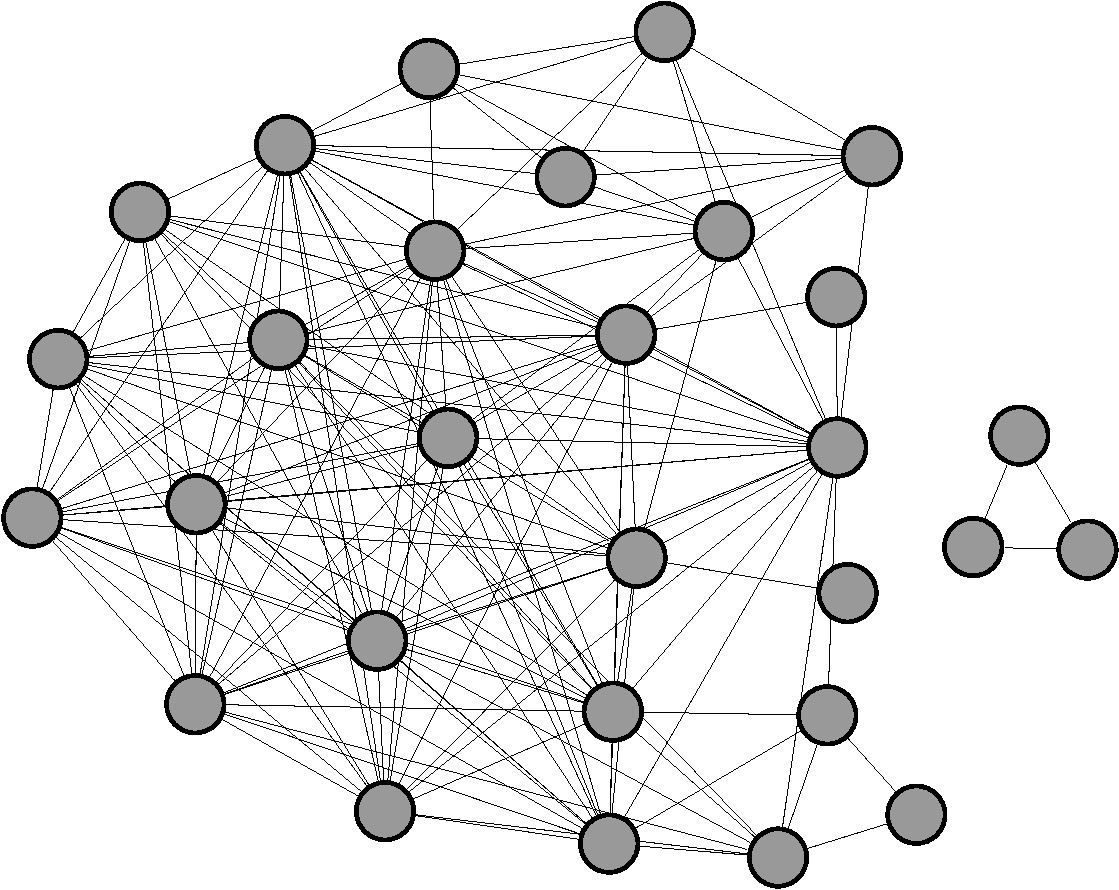
\includegraphics[width=\linewidth]{figures/disconnected-component-poldercast.pdf}
\caption{Visualization of disconnected component in the RINGS layer of PolderCast}
\label{fig:pold_disc}
\end{figure}

Another interesting use case for our tool is comparing different pub/sub systems and
protocols visually. Users may run the different systems using the same
workload, e.g.\ subscriptions and publications, and system parameters in
order to replay the execution and compare the different systems at
selected points in time. We include such comparisons in this chapter,
were we compare PolderCast and Scribe on a set of specific performance
metrics.

\section{Supported Performance Metrics}
\label{sec:metrics}



\section{System Architecture}
\label{sec:arch}

\begin{figure}[h]
\centering
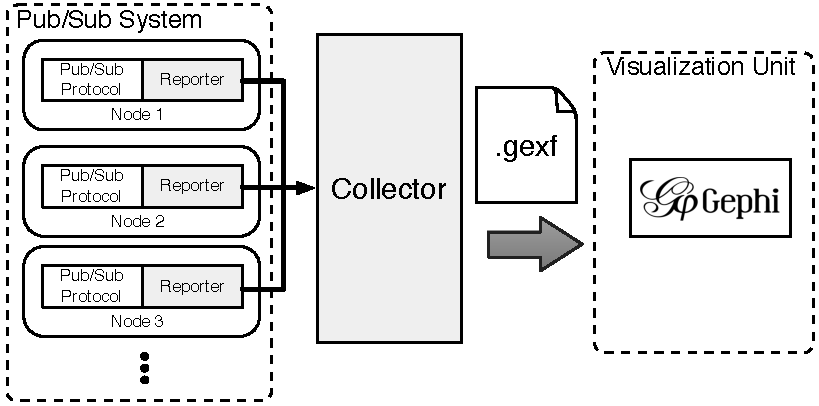
\includegraphics[width=\linewidth]{figures/arch}
\caption{Architecture diagram of \demo}
\label{fig:arch}
\end{figure}

The architecture of \demo~consists of three main components, all
depicted in Figure~\ref{fig:arch}: (1) \emph{Reporter}, (2)
\emph{Collector} and (3) \emph{Visualization Unit}.  The arrows seen in
Figure~\ref{fig:arch} depicts the flow of data in the architecture.
Each node in the executing system consists of a pub/sub protocol as well
as a ``Reporter''. The ``Reporter'' is the entity responsible for
providing the raw information required to compute various performance
metrics from the individual nodes participating in the overlay. This
information is pulled at regular intervals to a central site by the
``Collector'', which translates stores the information as a single
file in the \gexf{} format. This file is then interpreted by the
``Visualization Unit'', which consists of a single machine running
the Gephi tool. The Collector is designed to perform the collection of
data while in online mode, while the computation, aggregation and
derivation of various metrics is performed in in offline mode. The
Visualization Unit always operate in offline mode, as it waits for the
final report to be collated into a \gexf{} format for playback and
visualization.

The design of \demo~supports pub/sub systems that are deployed as
real distributed systems, as well as systems that are deployed in
simulation mode. This is due to the highly modular system architecture,
with strict separation of concerns, where the operation of both the
Collector and the Visualization Unit is separate from the reporting.
\demo~is designed to be a generic tool, where the only system specific
part of the architecture is the \emph{reporter interface} outlined in
Table~\ref{table:interface}. Any researcher or developer
who wants to use our framework only needs to provide an implementation
of this interface, which enables the Collector to retrieve the relevant
data from each individual node at the specified time points. These time
points are configurable, and all the information collected from the
reporter will in effect be the change of the system state from the last
time point with regards to the various performance metrics. We call
these time points \emph{reporting intervals}. The length of the intervals
is configurable, which provides the user with control over the
granularity of data collection, and thus the granularity of the
step-by-step replay of system execution performed in the Visualisation Unit. For example, if
running simulation using PeerNet, the user may determine whether or not
the reporting intervals should encompass several simulation cycles. Or,
in a real distributed pub/sub deployment scenario, the user can
determine the time delay between every reporting interval.


\subsection{Reporter}

The Reporter is responsible of providing the relevant data necessary in
order to calculate the desired performance metrics. In order to do so,
we specify a \emph{reporter interface} which is implemented at each
individual node participating in the pub/sub overlay. This interface
enables each nodes to log certain system parameters using its local
knowledge at each reporting interval. This local information is then pulled
by the Collector at the end of each reporting interval by invoking the
reporter interface. The available method calls and what data each method
returns is described in Table~\ref{table:interface}.

% ../tables/interface.tex
\begin{table}[h]
\centering
\resizebox{\columnwidth}{!}{%
\begin{tabular}{ll}
\toprule
Method Name                                       & Returns\\
\midrule
\tt long reportId()                      & The unique id of this node\\
\tt long[] reportNeighborIds()           & The unique ids of this node's neighbors\\
\tt long[] reportTopics()                & List of topic ids this node subscribes to\\
\tt long reportControlMsgsReceived()     & Number of overlay control messages received\\
\tt long reportControlMsgsSent()         & Number of overlay control messages sent\\
\tt long reportControlBytesReceived()    & Number of overlay control bytes received\\
\tt long reportControlBytesSent()        & Number of overlay control bytes sent\\
\tt PubMessage[] reportPubMsgsReceived() & Reports list of publication messages received\\
\tt PubMessage[] reportPubMsgsSent()     & Reports list of publication messages was sent\\

% \emph{reportDuplicatePubMessages(int topic, int messageId)} :  The number of duplicates received for a specific publication\\
% \hline
\end{tabular}
}%
\caption{Reporter Interface Methods}
\label{table:interface}
\end{table}



It is easy to see how the metrics mentioned in Section~\ref{sec:metrics}
can be derived from the methods listed in Table~\ref{table:interface}.
The structural properties of the overlay such as \emph{degree},
\emph{diameter} and \emph{clustering coefficient} can be derived by
reconstructing the overlay topology. This reconstruction can be achieved
through the two very first methods listed in
Table~\ref{table:interface}, namely \texttt{reportId()} and \texttt{reportNeighborIds()}.
For example, in our reporter interface
implementation for the RINGS layer in PolderCast, each node returns its
own id as well as the ids of both ring neighbors and random neighbors.
After this information is pulled, the Collector is able to derive a
graph structure where it first builds every node reported, and then draw
directed edges between these nodes based on the reported neighbor id
information. What topics each node subscribe to is also useful in order
to derive and visualize metrics such as \emph{Topic Diameter} and \emph{Subscription
    Size}. The Collector is able to pull information regarding topic
subscriptions through the \texttt{reportTopics()} interface method call.
Each node will return a set of topic ids, and the Collector is able to
use this information to attribute topics to each node, as well as edges.
In order to add topics to edges, the Collector simply iterates through
the topic id list of each node, and looks for a neighbor who share a
subscription to the same particular topic. A \emph{topic neighbor}. If a
topic neighbor of a node is found, the topic id is added as an attribute
to the edge connecting them. Applying topic attributes to nodes and
edges, provides the Visualization Unit with the ability to strip away
nodes and edges that does not belong to a particular topic, thereby
enabling calculation of topic diameter.

The dissemination properties of a given pub/sub system such as
\emph{hit ratio}, \emph{path lengths}, and number of duplicate publication
messages received can be derived by having each node provide a list of
publication messages sent and received. In order to calculate these
dissemination metrics, the publication needs to have a particular
structure. This structure is described in Table~\ref{table:structure}.
For example, in order to calculate hit-ratio for a specific topic, we
need to divide the number of subscribers of that topic who actually
received the message with the total number of topic subscribers. We
already know the which nodes subscribe to a particular topic through the
\texttt{reportTopics()} method call, and the list of publication
messages received by a node received can be retrieved through the
\texttt{reportPubMsgsReceived()} method call. Path lengths of a
message being published on a particular topic from a particular node may
be calculated in a similar fashion, as publication messages reported from
different nodes with the same id can be ordered based on their timestamp
values.

The number of duplicate publication messages received and sent by each
node is available through the \texttt{reportControlMsgsReceived()}  and
\texttt{reportControlMsgsReceived()} respectively, while the communication
overhead incurred by control messages in terms of bandwidth consumption can be
derived by the \texttt{reportControlBytesSent()} and
\texttt{reportControlBytesSent()} method calls.

% ../tables/pubmessage.tex
\begin{table}[]
\centering
\resizebox{\columnwidth}{!}{%
\begin{tabular}{ll}
\toprule
Message item           & Description\\
\midrule
\tt long  MsgId            & Unique id of the this message\\
\tt long  TopicId          & Topic id for which this message was generated\\
\tt long  SourceId         & Id of the previous hop node\\
\tt long  DestinationIds[]   & Ids of the next hop nodes\\
\tt long  OriginalSenderId & Node id of the message source\\
\tt long  TimeStamp        & Timestamp of the message sent/received\\
\end{tabular}
}%
\caption{Data Structure of a Publication Message}
\label{table:structure}
\end{table}



The structure of the publication messages outlined in
Table~\ref{table:structure} also allows for visualizing the paths of
publication messages. As, mentioned, this is one of the two types of
visualizations the Collector can output as a \gexf{} file (where the other
type is the overlay structure). In such a visualization the Collector
will look at the topic id of the message, and only include the nodes
interested in the particular topic in the visualization. The Collector
will then iterate through the messages sent and received by each node.
By analyzing the message further, the Collector is able to create
directed edges between the nodes which represent the path of the
publication message. The edges are dynamic, i.e.\ they include a Time
Interval attribute, enabling a step-by-step animation, where edges
appear as the animation is played back in the Visualization Unit,
tracing the path of the publication. This enables researchers,
developers as well as students to analyze publication dissemination
schemes hop-by-hop.

In addition to being able to configure at a chosen reporter interval,
users of this tool may choose to only report partial information. For
example users may choose to only report structural information such as
node ids, or only dissemination specific data such as publication
messages sent and received. This flexibility is useful if only a few
aspects of system performance need analysis.

\subsection{Collector}

The Collector is the component responsible for pulling information from
the nodes at every reporting interval. It is also responsible for
aggregating and calculating certain custom metrics. By custom, we mean
any metric that is not included in the Gephi statistics component. These
metrics are usually related to dissemination and include hit-ratio,
duplicate publication messages received and path lengths. Metrics
related to overlay structure can be calculated in Gephi. These metrics
include degree, clustering coefficient, diameter and centralities. Topic
Diameter however, is a special case. In order to calculate topic
diameter, the graph needs to be filtered down to a subgraph which only
includes nodes and edges for a given topic and calculate the metrics for
every such subgraph. To do this manually using
the Gephi GUI-client would be an time consuming and error-prone task.
Therefore, the Collector  leverages the Gephi Toolkit in order to
automate this task. The collector supports what the Gephi community
refers to as \emph{static} and \emph{dynamic} metrics. This is also
referred to in literature and in~\cite{korsveien2014vizpub} as
\emph{instantaneous} and \emph{aggregated} metrics. In this thesis, we
will refer to them as static and dynamic, in order to be consistent
with the terminology used by the Gephi community. In short, static
metrics pertains to a specific point in time, while dynamic metrics is
based on historical values. The statistics component in Gephi includes
both type of metrics, but dynamic metrics only include degree and
clustering coefficient, while the Collector is able to compute dynamic
metrics for all properties such as centralities, hit-ratio and number of
control messages sent and received.

Aggregation of data is performed by serializing each individual report received
from the reporters into temporary files which are stored on disk. The
collector will then iterate through these files and output a final
report using the \gexf{} file format. While collection is done in online
mode, aggregation is performed in offline mode. The offline aggregation
of data prevents the collector from acting as a bottleneck. Indeed, the
collection and aggregation of data is highly decoupled from the
execution of the pub/sub protocol itself. As an alternative,
the Reporters are also able to log reports locally, and push them to
the collector at the end of pub/sub execution.

The Collector will use the information pulled from the reporters in
order to apply attributes to nodes and edges. These attributes form the
basis of node labels and colors in Gephi. For example, number of
control messages sent is a node attribute which can be represented as a
numeric label on nodes. Also Gephi will inspect all nodes for their
``control messages sent'' attribute value, and determine the maximum and
minimum value. These value form a value range which can be used to color
the nodes on a gradient. For example, the closer a nodes value is to the
maximum, the deeper the color of the node.

Some of the attributes are derived from the reported information, such
as \emph{subscription size}, which is derived from the length of the
collection returned by \texttt{reportTopics()}. What attributes to apply
is configurable. The only edge attributes supported by the Collector is
the topics attribute. This is derived by determining the set of
subscribers of a topic and analyzing the edges between them. If two
nodes have an edge between them, they are topic neighbors. The list of
node attributes supported is far more extensive and includes:

\begin{itemize}
    \item Control messages sent
    \item Control messages received
    \item Control messages sent in kilobytes
    \item Control messages received in kilobytes
    \item List of topics subscribed to
    \item Number of topics subscribed to (i.e.\ \emph{Subscription Size})
    \item Number of duplicate publication messages received
\end{itemize}

These attributes describe data pertaining to individual nodes. However,
the Collector will also calculate data which is global to the entire
graph. For example, the collector is able to calculate the average value
for numeric attributes, such as control messages sent for each interval.
The collector iterates through the interval range, and sums the numeric
attribute value of each node that exists in this interval and divide
this number with the number of existing nodes. The resulting averages
are applied to all nodes as labels, even though they represent a global
value, i.e.\ it is not a value specific to the particular node. This is a
workaround, as Gephi does not support displaying graph attributes.
Currently, the global values calculated by the Collector includes:

\begin{itemize}
    \item Hit-Ratio
    \item Average Number of Control Messages Sent
    \item Average Number of Control Messages Received
    \item Average Number of Control Messages Received in kilobytes
    \item Average Number of Control Messages Received in kilobytes
\end{itemize}

The Collector is also able to calculate average intended for
plotting time series using a tool such as gnuplot, rather than be
applied as a node label. Adding support for
these averages as node attributes is not a priority at this point, but
will be implemented in the near future. We describe the supported
calculations in
Section~\ref{sec:viz_eval}, where we further describe the use case
intended for this feature of \demo.

\subsection{Visualization Unit}

The Visualization Unit is a machine running the Gephi Open Graph Viz
tool. This tool is able to interpret the \gexf{} file generated by the
Collector and visualize the execution of the pub/sub system in question.
Gephi provides a rich GUI-experience where the user may interact with
the graph representation, apply layout algorithms, filter the graph
, execute metrics, apply color and size based on graph
properties and animate the graph evolving over time through the timeline
component. The Gephi software architecture is highly modular and
supports extensions via plugins, some of which are available in a
official plugin marketplace found at~\cite{gephimarketplace}. New
metrics, filters or database support may be implemented through such
plugins by developers and published to the marketplace free of charge.

Gephi provides many tools and components which are useful in the context
of researching and analysing pub/sub overlays:

\begin{figure}[h]
    \centering
    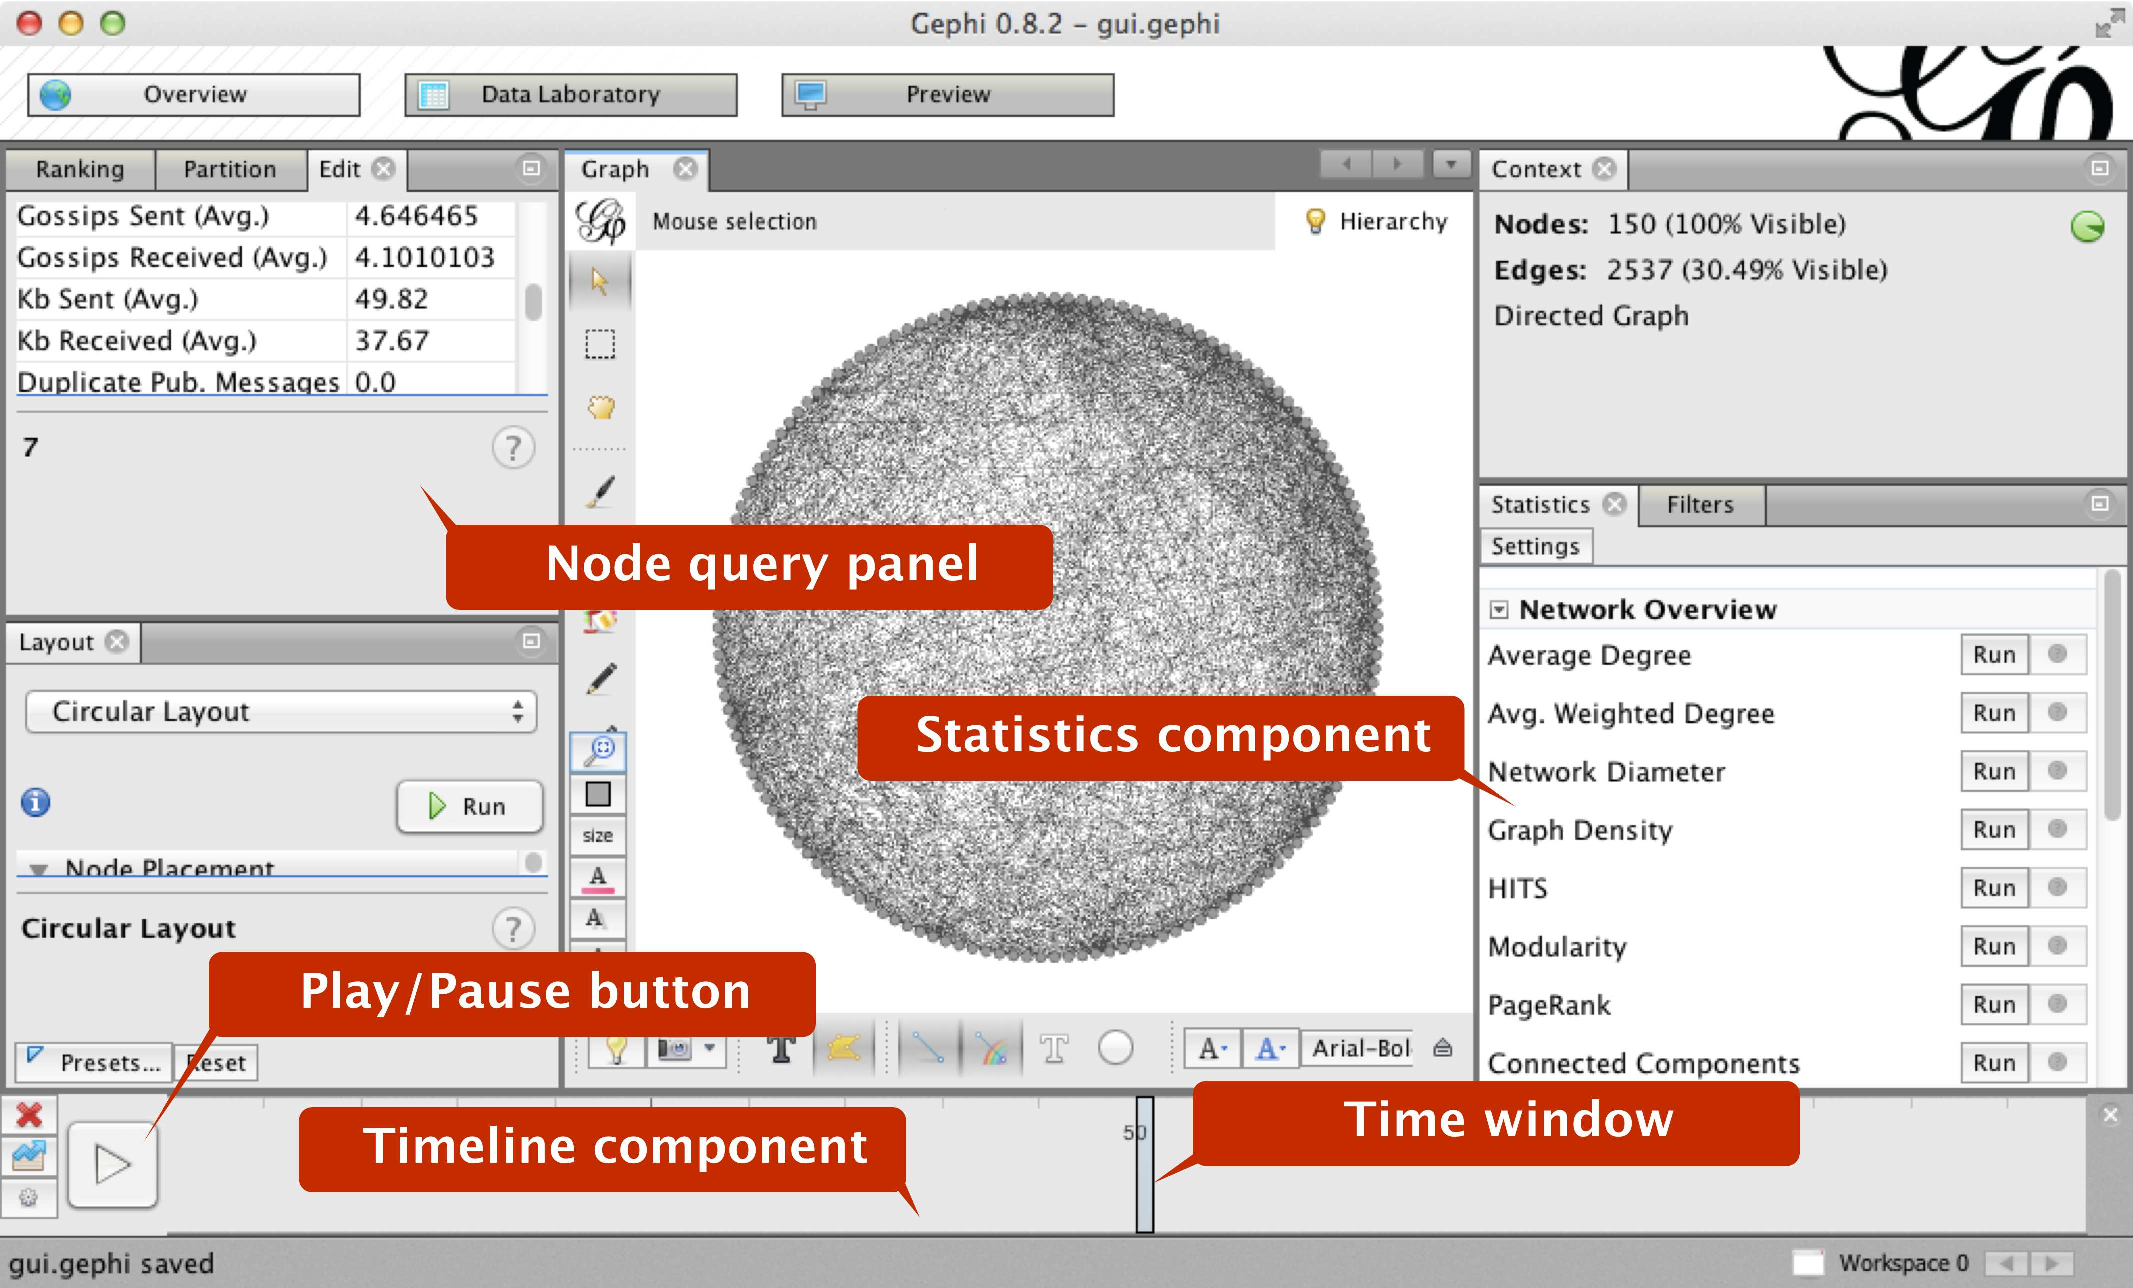
\includegraphics[width=\textwidth]{figures/gui_ann}
    \caption{Snapshot of Gephi GUI with several important components
        annotated}
\end{figure}

\begin{description}

\item[Node and Edge pencil tools] \hfill \\

    These two tools enable the user to create nodes and edges by
    clicking in the graph view. Edges can be undirected or directed,
    where direction is indicated with an arrow. These two tools combined
    enables building a graph by hand.

    Building such graphs can be useful in order to reason, analyze or
    learn network algorithms such as event dissemination algorithms.
    For example, the user can start with a single node which can act as
    the event source, and build the topology as the event disseminates,
    carefully following the particular algorithm in question when doing
    so. The user can also add attributes to the nodes and edges either
    through the node query tool or in the Data Laboratory component
    which also aids in visualising and understanding properties,
    drawbacks and advantages of such algorithms.

\item[Node Query Tool] \hfill \\

    \begin{figure}[h!]
        \centering
        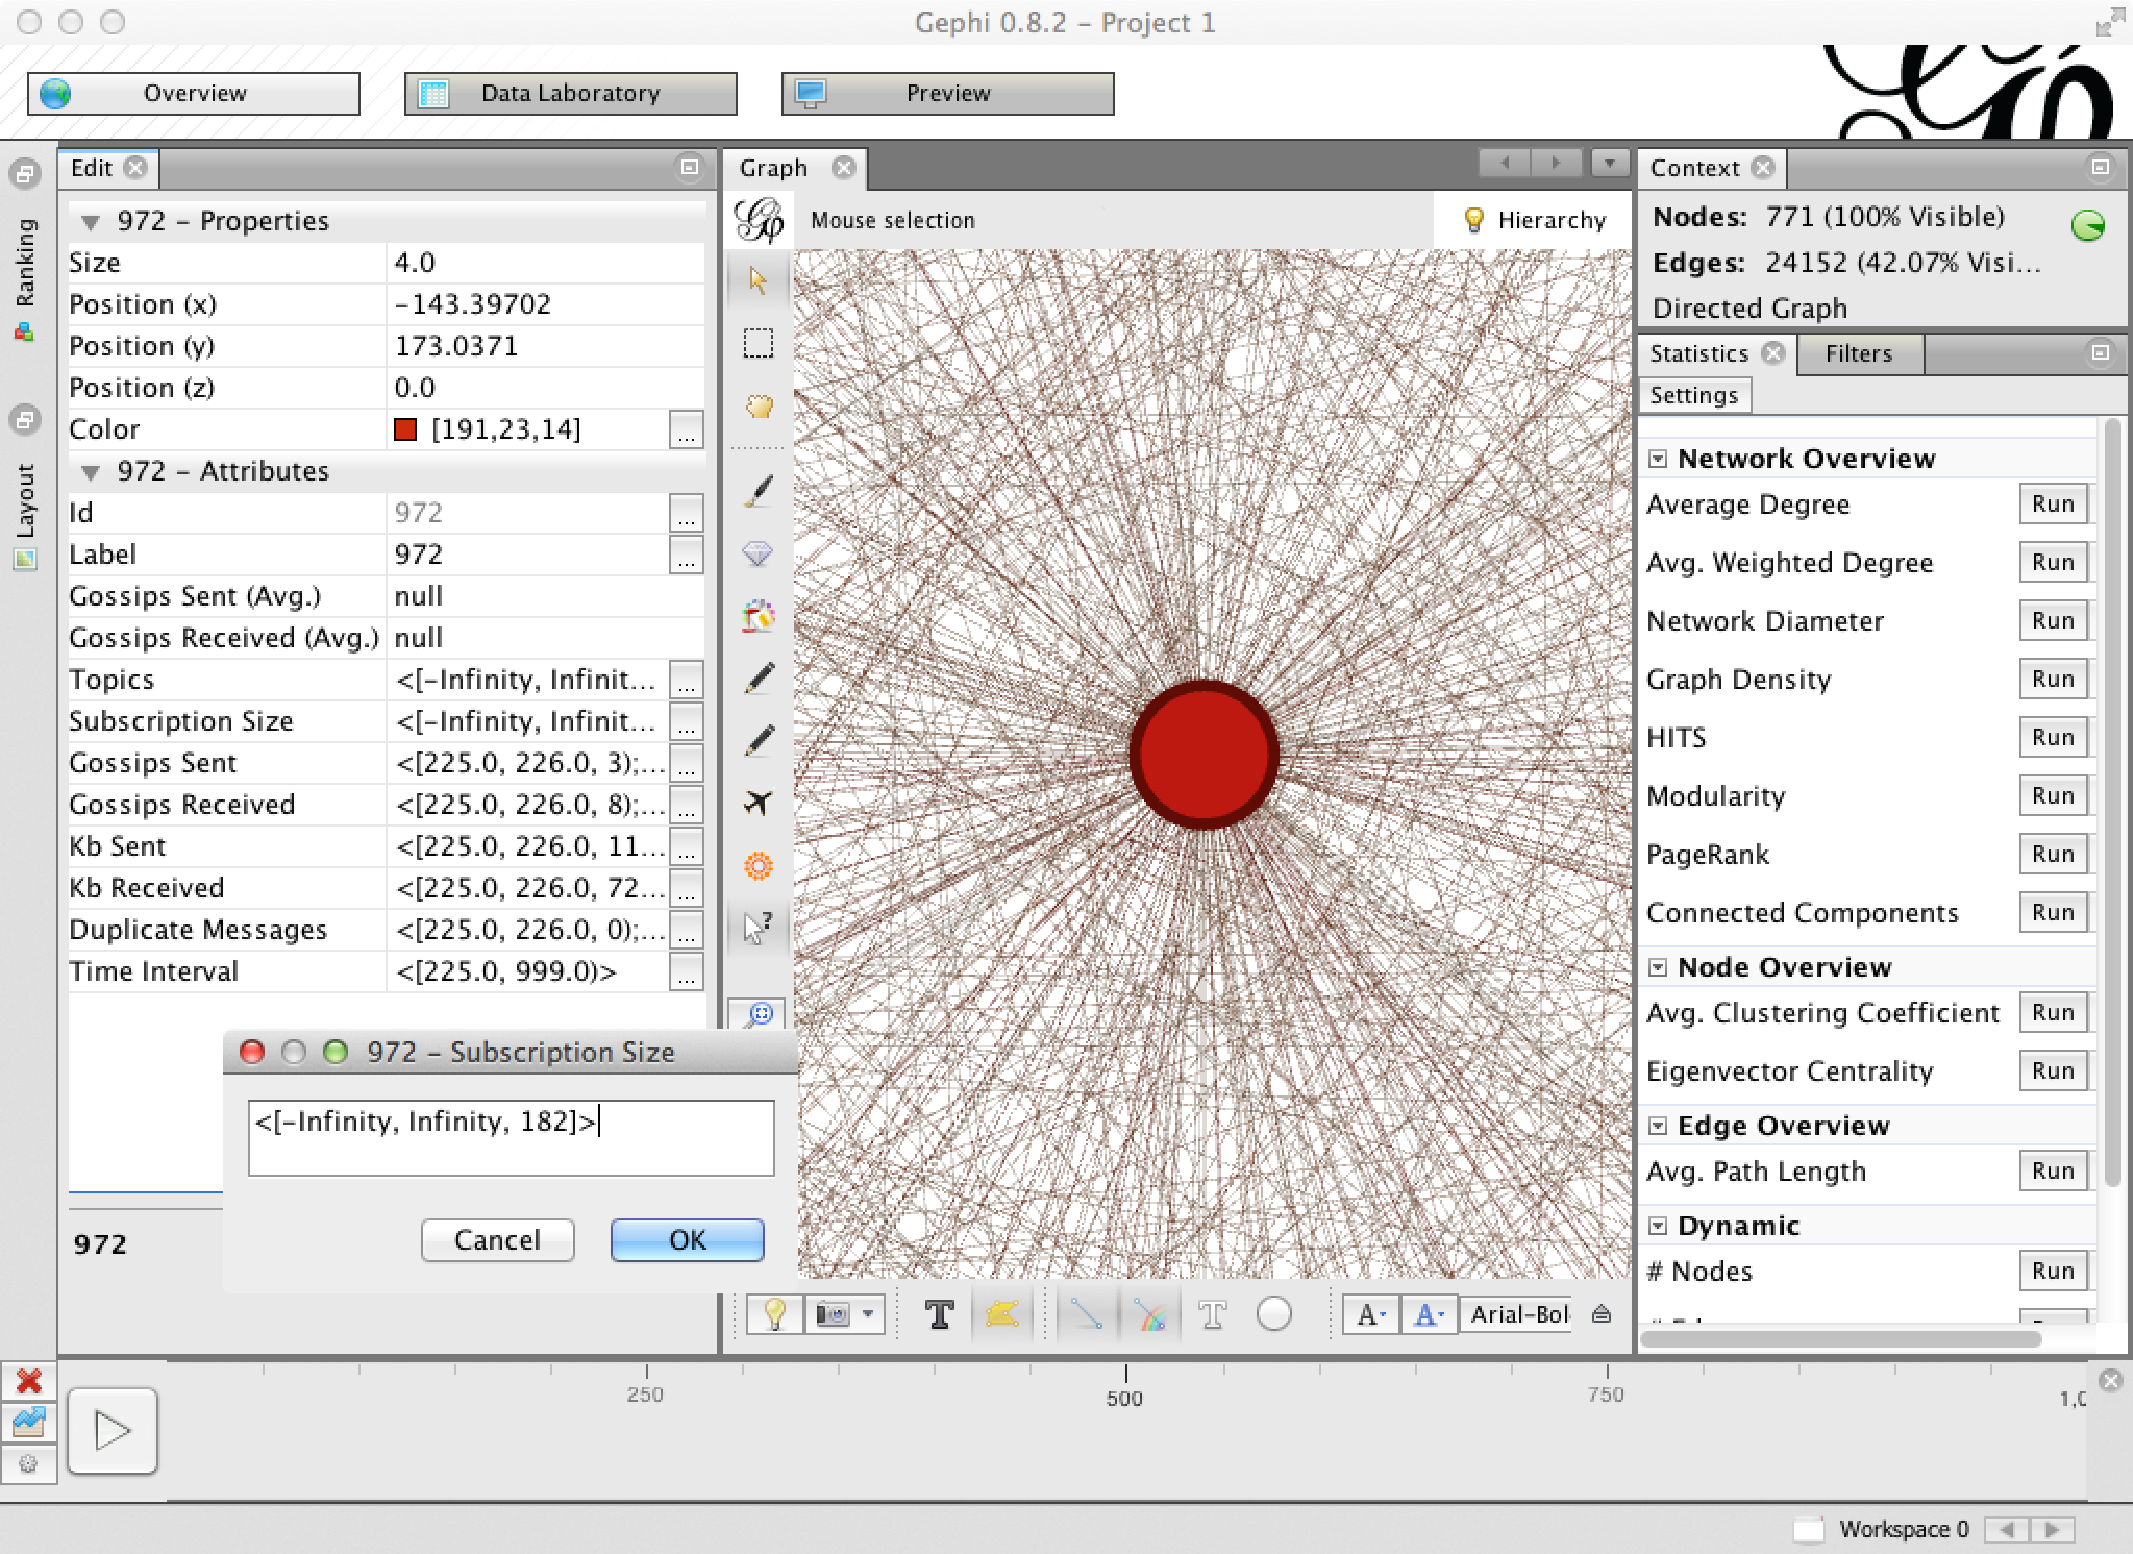
\includegraphics[width=\linewidth]{figures/gui_node_query}
        \caption{The Node Query Tool opens a panel (to the left) that can be used to inspect the
            attributes of a node, here it is used to inspect the
            subscription size of a high-degree node}
        \label{fig:gui_node_query}
    \end{figure}

    With the Node Query Tool the user is able to click on a node on the
    graph model, and a panel will appear to the left with information
    regarding the properties and attributes of this node. Properties include
    data describing the visual properties of the node such as size, position
    and color, while attributes include the id and label and Time Interval
    attributes and any additional user defined attributes. In our case, such
    user defined attributes would include topics, subscription size and
    number of control messages sent and received. In
    Figure~\ref{fig:gui_node_query}, the Node Query tool is used to
    inspect the subscription size (i.e.\ number of topics the node
    subscribe to) of a high-degree node.

    Both the properties and attributes of the node are editable through this
    panel view. The user can select a property to change the visual
    representation of the node, or the attributes to change their value. The
    time interval attribute is interesting to edit in particular as it
    represents the points in time in which a node exists in the graph model.
    One example scenario is editing the time interval attribute for a certain
    nodes in order to see how it affects a particular metric as well as the
    overlay topology.

\item[Shortest Path Tool] \hfill \\

    With the shortest path tool selected, the user may click on two nodes on
    the graph model, and if there is a shortest path between them, this path
    will be highlighted with a color. This is useful in order reason about the
    relationship between key nodes in the graph, or to compare shortest path
    between several pairs of nodes.

\item[Heat Map Tool] \hfill \\

    The heat map tool enables the user to click on a node in the graph model
    and color its neighborhood based on the edge weight distance between
    them. More specifically, it sets the node color intensity lower for more
    distant nodes and stronger for nodes that are closer. Edge weight is a
    standard edge attribute that are by default set to 1. This means that in
    the default case, the visualization will represent the hop count
    distance from the particular node selected by the user. However, the
    edge weight can be edited by the user in order to represent other
    properties of a system. As an example, imagine setting the edge weight
    to represent network latency between two nodes. In this case, a
    neighboring node which is adjacent to the selected node would have a
    lower color intensity if the latency between them is higher than another
    neighboring node which is further away in terms of hop count.

\item[Timeline Component] \hfill \\

    The timeline component introduces an animation scheme for dynamic
    graphs. The user may choose playback parameters such as time
    interval size, step size and playback speed. The time interval will
    filter out a subgraph defined by the upper and lower bound of the
    interval. The evolution of the dynamic graph will then be animated
    by moving these bounds by the distance defined by the step
    parameter. The delay between each step is decided by the playback
    speed.

    The timeline enables the user to visually inspect the change in
    graph topology over time, as well as visualize and inspect node and
    edge attributes of the graph through both color, size and text
    labels which is able to change dynamically as part of the graph
    model animation. The timeline also enables jumping to a specific
    point in time and investigating the corresponding subgraph and its
    properties by changing the upper and lower bound of the time
    interval.

\item[Statistics Component] \hfill \\

    The metric component enables graph topology analysis by executing
    metrics on the graph. There are two types of metric algorithms in Gephi:
    static and dynamic. Static metrics are only able to execute on graph
    model representing a single point in time, while dynamic will traverse
    the time line by executing the metric iteratively across a set of time
    intervals. When executing a dynamic metric, the user is able to choose
    window size and time step. The window size is a time interval which will
    be moved by the step size defined by the user. Metrics are divided
    into \emph{static} and \emph{dynamic} metrics, where the former
    calculates a single value based on the currently defined time
    window, while the latter calculates a time series of values. When
    executing a dynamic metric, the user must define the time window
    size, and tick. The have the same functionality as step parameter
    when using the timeline component. When the metric executes,
    the time window will iterate through the entire time range of the
    simulation, calculating a static metric at each step. When finished,
    a time series is plotted and displayed for the user.

    The Statistics component include several metrics which are relevant
    to pub/sub overlays. Useful static metrics include, but are not
    limited to:

    \begin{itemize}
        \item{Degree (In/Out/Avg./Max/Min/Distr.)}
        \item{Avg. Cluster Coefficient}
        \item{Centrality (Beetweeness/Closeness/Eccentricity)}
        \item{Average Path length}
        \item{Radius}
        \item{Network Diameter}
        \item{Number of Shortest Paths}
    \end{itemize}

    Out of these, only degree and the clustering coefficient metrics have dynamic
    versions, where both calculates the average value over time. The
    average for dynamic metrics are calculated by dividing the sum of
    all node attribute values with the total number of nodes in both
    cases.

\item[Ranking Component] \hfill \\

    The ranking component is a key feature of Gephi which enables
    visualization based on node or edge attributes in form of color
    and size. When coloring nodes or edges, the ranking component
    will apply a gradient over the range of attribute values. The
    ranking component also include a result list, where the user may
    sort nodes based on the specified attribute value, which is
    useful for quickly finding the nodes with maximum value and
    minimum value. This is helpful for identifying bottlenecks in
    the system or potential load balancing issues.

    The ranking component also includes an auto apply feature, which
    supports visualising attributes dynamically while playing back the
    graph via the timeline component.

\item[Layout Component] \hfill \\

    The layout component enables the user to execute algorithms that
    calculates the position of the nodes. The user is able to adjust the
    parameters of these algorithms in order to manipulate the visual
    layout. The different algorithms emphasize different aspects of the
    topology. One example is the Force Atlas layout algorithm which
    simulates the effect of gravity on the nodes, where linked nodes
    attract each other and non-linked nodes are pushed apart. This
    particular algorithm is useful for visually detecting clusters and
    communities. Another useful algorithm is the Circular Layout
    algorithm, where nodes are positioned in a circle ordered on a
    specific attributes selectable by the user. This is useful in order
    to visualize node rankings on particular attributes.

\item[Filter Component] \hfill \\

    Filters may be applied to the graph in order to strip away nodes or
    edges on the basis of their attributes which also includes any
    calculated metrics. Filters may strip away nodes based on a value range if
    the attribute type is a number, or a regex match if the attribute is
    a string. Filters can also be combined through special operator filters
    representing set operations such as union and intersect.

    Filters are an essential mechanism in order to analyze subgraphs.
    One use example is the case of calculating topic diameters in pub/sub systems,
    where a subgraph can be filtered on a topic attribute. This
    allows executing the diameter metric on the resulting subgraph
    on the selected topic.

\item[Data Laboratory Component] \hfill \\

    The Data laboratory component enables the user to work with the node
    and edge attributes of the graph. This component provides the user
    with separate table views of node and edge attributes. Each row in
    these table represent a node or edge, and each column an attribute
    for that particular node or edge. Columns may be added or removed by
    the user. The data laboratory also provides functionality for
    manipulating columns such as merging two columns or creating new
    columns based on data from selected columns. Attribute data in
    columns that are static (i.e.\ has no lower or upper time interval
    bound associated with them) can be converted to dynamic through this
    component. Also, resizing or coloring all edges or nodes is possible
    through the laboratory by selecting all rows and right-clicking. In
    addition to this, the data laboratory also enables the user to export the
    data to file for further statistical analysis.

\end{description}

\section{Examples of Visualizations}

In this section, we present a number of visualization produced by \demo.
The examples we provide in this section include both visualizations of
overlay structure as well as hop-by-hop message dissemination.  We
implement a reporter interface both for PolderCast as well as Scribe and
provide examples of visualizations for both protocols and compare them
visually on various performance metrics. Both protocols are implemented
using the PeerNet P2P simulator by updating existing PeerSim
implementations of Scribe and PolderCast.

Many of these visualizations were part of our demonstration at
DEBS 2014, and should provide some insight the benefits of using
our tool, and what sort of possibilities there are in terms of
visualizing overlays.

\subsection{Data Traces Used in Simulations}

We use publicly available datasets from
Facebook\cite{facebook-eurosys09} and Twitter\cite{Kwak10www}. The Facebook
dataset consists of 3 million user profiles along with 28.3 million
social relations between these users. The Twitter dataset consists of
41.7 million distinct user profiles and 1.47 billion follow/followed
relations. In both datasets users are modeled as topics. In the Facebook
dataset, subscriptions are modeled after the friend list of that user.
As relationships are bidirectional, two topics will subscribe to each
other. In Twitter, relationships are unidirectional, as users may choose
to follow other users, and no user who is followed need to reciprocate.
As a user is modeled as a topic, its list of followers are modeled as
the subscribers of that topic. The simulations we run in this chapter
consists of 2000 nodes, where the workloads have been extracted in~\cite{Setty:2012}.

Churn is based on the Skype super-peer network data
trace~\cite{Guha:2006}, where 4000 nodes are tracked for joining and
leaving timestamps for one month staring on September 12, 2005. Finally,
we use the King dataset~\cite{king} in order to model latency between
nodes.

\subsection{Overlay Evolution During Churn}
\label{sec:churn}

\begin{figure*}[h]
    \centering
    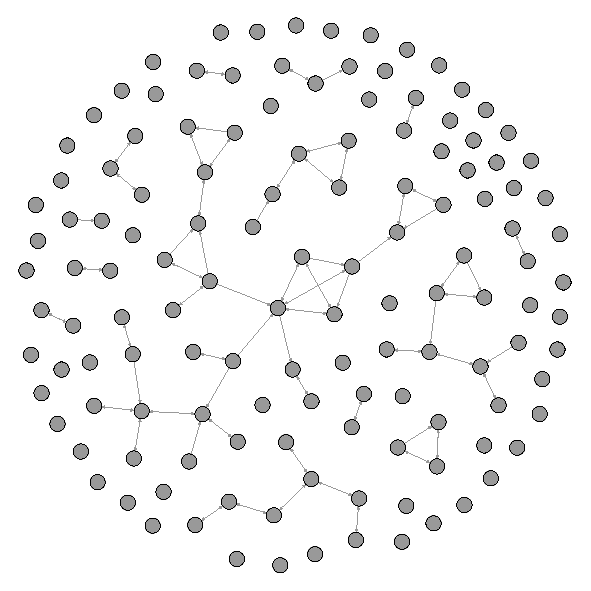
\includegraphics[scale=0.35]{figures/churn_0}
    \caption{Overlay structure of PolderCast at interval 0}
    \label{fig:churn0}
    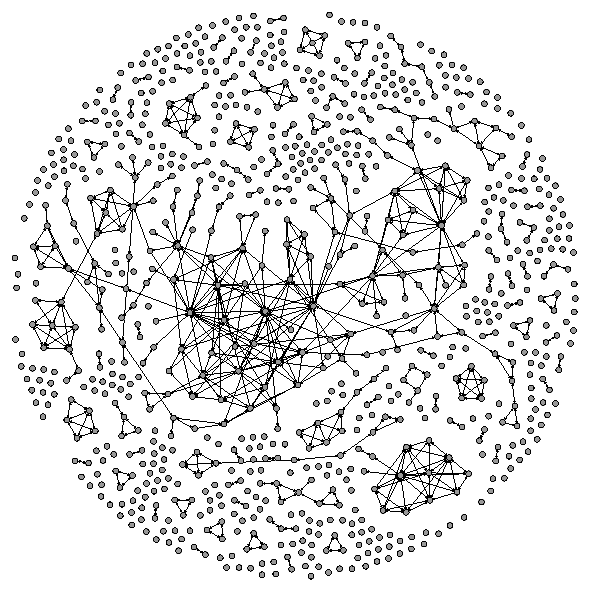
\includegraphics[scale=0.85]{figures/churn_250}
    \caption{Overlay structure  of PolderCast at interval 250}
    \label{fig:churn250}
    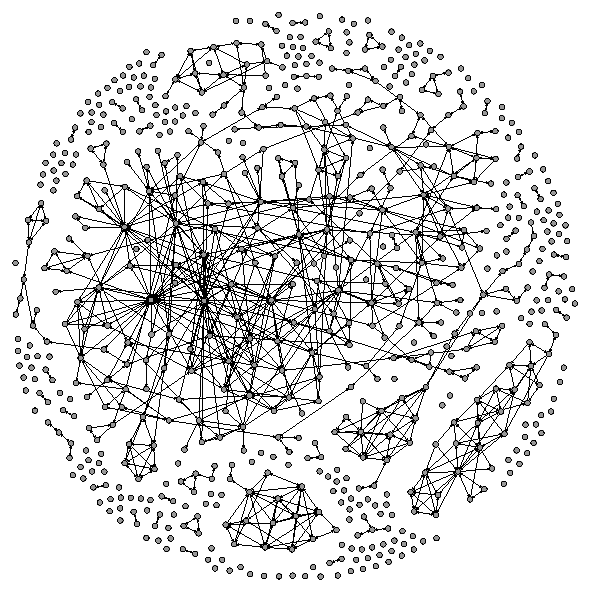
\includegraphics[scale=0.85]{figures/churn_500}
    \caption{Overlay structure of PolderCast at interval 500}
    \label{fig:churn500}
\end{figure*}

In Figure~\ref{fig:churn0},~\ref{fig:churn250} and~\ref{fig:churn500} we
visualize the overlay topology of 2000 PolderCast nodes during churn.
This is one of the examples of visualizations we presented at DEBS 2014.
Each figure corresponds to a reporter interval. Figure~\ref{fig:churn0}
depicts the overlay at interval 0, where 132 nodes are up while the
remaining 1868 are down due to churn. The snapshot in
Figure~\ref{fig:churn250} depicts the overlay at interval 250, after a
considerable number of nodes have joined the network. More specifically,
interval 250 consists of 1028 nodes, which means 896 nodes joined in the
interim. The edges are also evolving. While the first interval consisted
of 108 edges, interval 250 consists of 1028 edges. It is interesting to
see the edges evolve over time, as they provide can provide us with
immediate visual feedback on properties such as clustering of nodes,
graph density and node degree. Such properties can then be further
analyzed using the Statistics component in Gephi.

Furthermore, such visualizations might provide immediate information
regarding the dataset being used. As mentioned in
Section~\ref{sec:overview}, we encountered a scenario where an artefact
in the dataset resulted in a disconnected component in the visualized
overlay. Here we notice that many of the nodes are disconnected. This is
due to a sampling bias, as the Facebook dataset contains 10,000 nodes
while the simulation runs 2000 nodes. However, visualizations including
such a high number of nodes is not appropriate for print due to space
restrictions.

\subsection{Visualizing Performance Metrics}

\demo{} supports visualizing a number of performance metrics. These
metrics are applied as attributes both to nodes and to labels. Here we
will take advantage of these capabilities and present a range of
visualizations for PolderCast, in order to determine what we can learn
from them.

\subsection{Publication Message Dissemination}
\label{sec:dissviz}

\begin{figure*}[h]
    \centering
    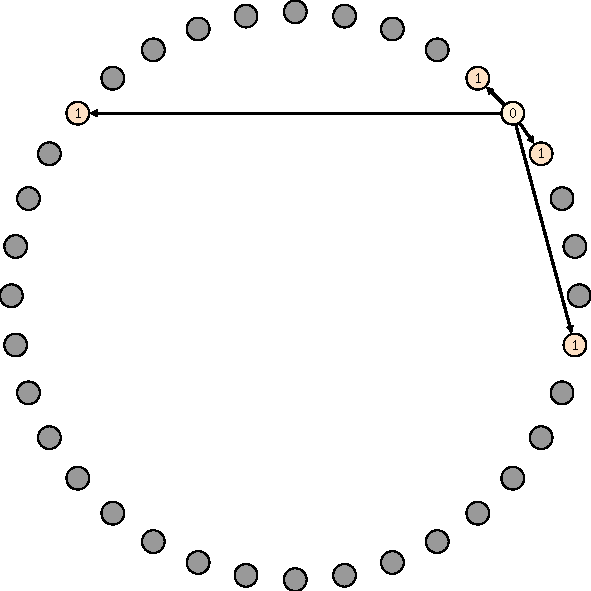
\includegraphics[scale=0.5]{figures/diss_1}
    \caption{Visualization of the first message dissemination hop}
    \label{fig:diss_1}
    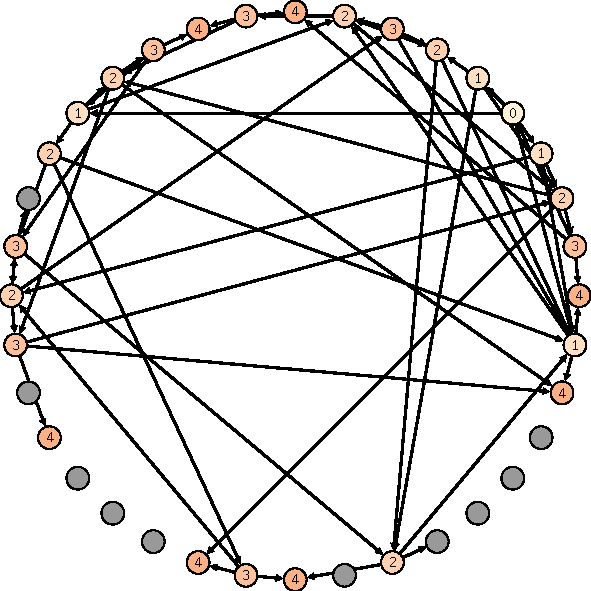
\includegraphics[scale=0.5]{figures/diss_2}
    \caption{Visualization after 4 hops}
    \label{fig:diss_2}
\end{figure*}

In subsection~\ref{sec:churn} we illustrate one of the two types of
visualizations it is possible to produce by leveraging \demo. Here we will describe the second:
event dissemination visualizations.

We run a PeerNet simulation in distributed mode with 100 nodes running
the PolderCast protocol with a fanout set to $f=2$. In order to scale
the experiment, the simulation includes 10 machines, where each machine
is running 100 PeerNet nodes.  We publish a single message on the
most popular topic which includes 63 subscribers. By analyzing copies of
the publication message received on each node, the Collector is able to
create a step-by-step visualization where directed edges are drawn as
the message is disseminated through the overlay.  These edges depict the
path of the message being disseminated. The visualization includes 189
edges in total, which indicates how many publication messages was sent
by all nodes during the simulation.

Figure~\ref{fig:diss_1},~\ref{fig:diss_2} and~\ref{fig:diss_3} are
snapshots of the dissemination visualization after hop 1, 4 and 7
respectively. The nodes have been arranged in a ring using the Layout
component in Gephi. Also they are ordered by node id, making it easier
to see whether an edge represent a ring link or a random link. The
labels indicate the hop number of the message received by that node. On
the left side of the ring there is a node with the label ``0'', which
indicates that this is the publishing node. A node with the label ``1'',
means the node received a message at the first hop, a node with a label
``2'' that it received a message at the second hop, and so on. In
addition to numeric labels, the nodes are color coded on a gradient. The
deeper the color of the node, the higher the hop count, which means it
is further away from the publisher. In figure~\ref{fig:diss_3} the node
furthest away is easily spotted on the left by its deep red color. This
is the last node to receive the publication.

It might seem strange that the last node to receive the message is an
immediate ring neighbor of a node who received the message on the first
hop. Observe that in Figure~\ref{fig:diss_1} this neighboring node who
received a message on the first hop does indeed send a message to the
node in question. However, in Figure~\ref{fig:diss_2}, which depict the
dissemination after the message has been sent, no numeric label is
applied to the node. This could bear the impression that this note did
not receive any message, however this is not the case. The explanation
behind this is latency. The latency between these two nodes is so high
that by the time it received the message from its ring neighbor, the
message was already received from somewhere else. We choose to visualize
this by drawing an edge to the node and then refrain from applying a
numeric label. When we reach the point in the animation where this node
receives a message for the first time, we apply the hop count of this
message as a numeric node label.

When inspecting the dissemination algorithm of protocols visually,
implementation details which could otherwise be overlooked become easily
detectable. For example, in Figure~\ref{fig:diss_1} it can be observed
that the publisher node sends a message to four nodes, even though the
fanout is set to $f=2$.  This fanout should indicate that the node
should send the message to three neighbors, based on the description of
the dissemination algorithm of PolderCast, summarized in
Chapter~\ref{ch:background}.  However, there is an implementation detail
in PolderCast that is not mentioned in the original
paper~\cite{Setty:2012}. In the implementation of the PolderCast
protocol, publishers send messages to one additional random node in
order to boost the initial phase of the dissemination. Learning such
implementation details is useful to both researchers and developers, and
it is especially useful for students. We believe \demo can be very
valuable as an educational tool, as its grant students with the
capability of controlling the dissemination by using the Timeline
component in Gephi. Students may pause the visualization at any point in
time or jump to any step of the visualization in order to fully
understand the benefits and drawbacks of the particular dissemination
scheme being studied.

It is also useful to create such visualizations in order to discover
issues or bugs with the dissemination algorithm. As observed in
Figure~\ref{fig:diss_1}, the publisher disseminates to four nodes, where
two of these should be random neighbors. However, the publisher
seemingly sends the message to three of its closest ring neighbors.
This means a neighbor close to it might have been chosen as a random
neighbor. This might indicate a bug in the CYCLON module of PolderCast,
which is responsible of providing the RINGS layer with uniform random
neighbors.  However, the dissemination happens at an early point of the
experiment, more specifically, after 50 PeerNet cycles. Due to
experimental settings, this might not have been enough time for the
different layers of overlay in PolderCast to converge. Also, it could be
a special case, which resulted in the publisher being a bit unlucky when
picking a random neighbor in this particular scenario. Regardless,
visualizing dissemination leads to these interesting observations, which
might lead to even more interesting findings with regards to protocol
behaviour.  One such interesting observation is how a fanout of $f=2$
leads to a special case when dissemination messages in PolderCast. More
specifically, as mentioned in Chapter~\ref{ch:background}, a node
running PolderCast will forward a message to both ring neighbors and
$f-2$ random neighbors if it received a message through a random link.
But if $f=2$, then $f-2 = 0$. However, PolderCast will always include a
random link when it forwards a message, meaning that the number of
random neighbors any node will forwards a message to is set to a minimum
of one. This is yet another implementation detail which could be hard to
catch without being able to inspect the dissemination protocol visually.

One of the trade-offs we mention in Chapter~\ref{ch:design-challenges}
is the one between the number of duplicate messages received and the
robustness of message delivery. In Figure~\ref{fig:diss_3} we can
quickly confirm visually that some of the nodes have a high degree. This
indicates that the number of duplicate messages this these nodes
received is high. A certain number of duplicate messages in epidemic
dissemination is to be expected, but a balance should be struck between
number of duplicate messages and reliable delivery. If there are too
many unnecessary messages being sent, scalability in terms of bandwidth
suffers.

Deriving the exact number of duplicate messages received by each node is
trivial. As each directed edge represent  a message being sent, all we
need to do is calculate the in-degree of each node using the Statistics
component in Gephi. The result can be seen in Figure~\ref{fig:dups}.
This visualization indicate that PolderCast does indeed introduce a
rather high number of duplicate messages being received on each node.
However, it is only an indication and nothing more as this visualization
traces a single publication message on a single topic. However, such
an indication can be useful in order to guide researchers and developers
towards potential issues or bugs. We believe \demo is a useful tool in
this aspect.

\begin{figure*}[h]
    \centering
    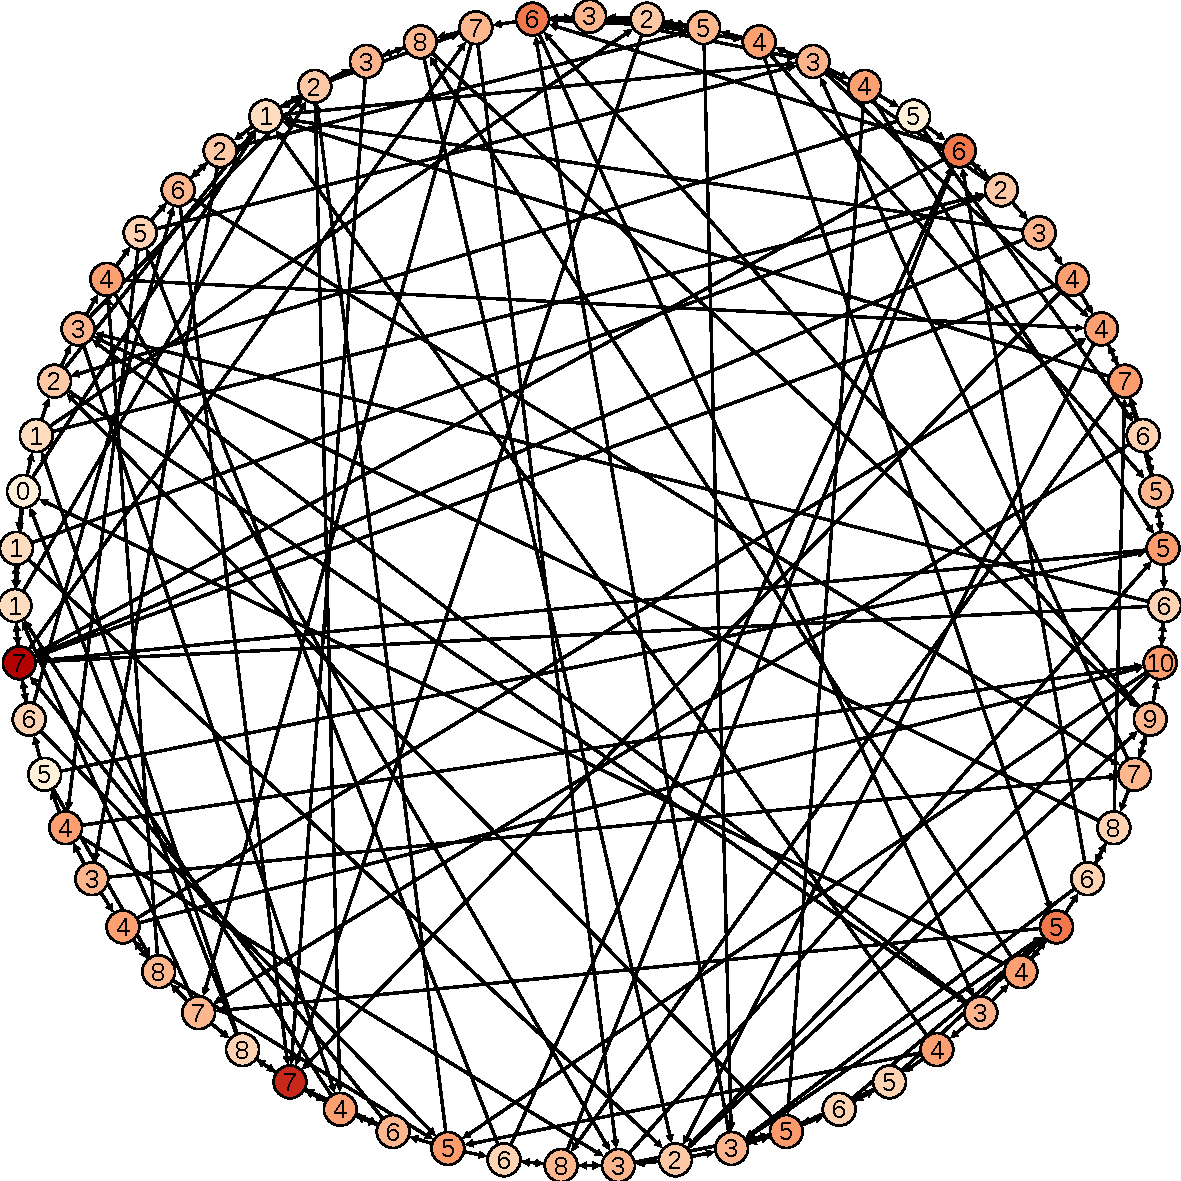
\includegraphics[scale=0.5]{figures/diss_3}
    \caption{Visualization of PolderCast after the end of dissemination}
    \label{fig:diss_3}
    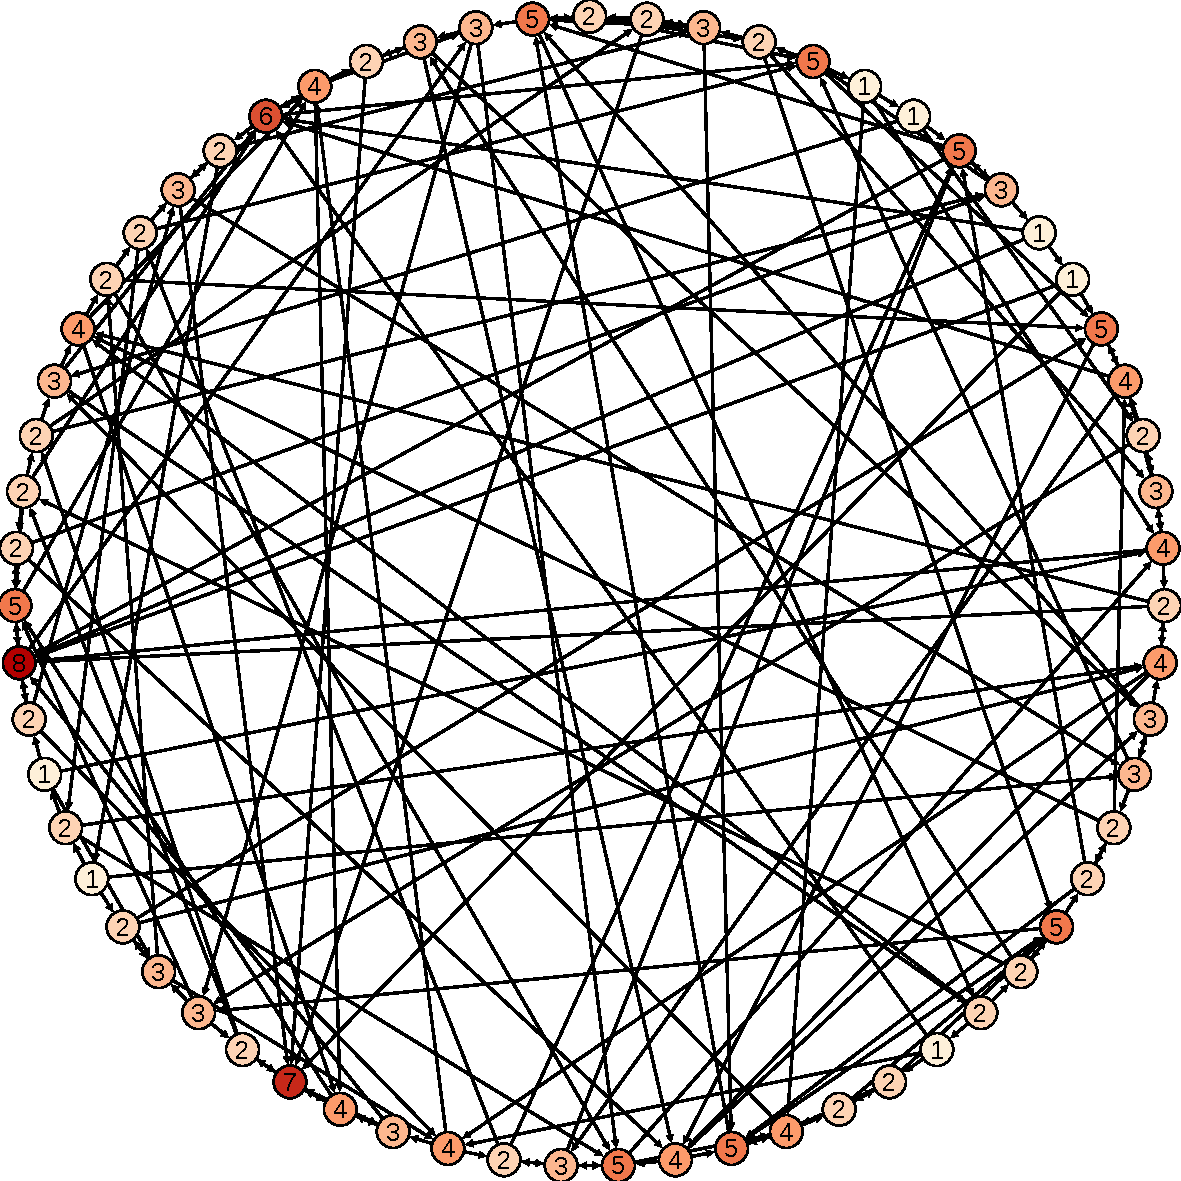
\includegraphics[scale=0.5]{figures/diss_dup_msg}
    \label{fig:dups}
    \caption{Visualization of duplicate publication messages received by
    each node in PolderCast}
\end{figure*}

\subsection{Comparing Pub/Sub Systems Visually}

\section{\demo as a Framework for Evaluating Pub/Sub Systems}
\label{sec:viz_eval}

In addition to outputting a \gexf file which can be used to produce
visualizations in Gephi, The collector is also able to generate \csv
files which can be used to plot a time series of metrics such as degree,
clustering coefficient and centralities. Each time point in the time
series will represent a \emph{Reporter Interval}. Although the Data
Laboratory component in Gephi is able to output such \csv files, it is
much more convenient to output them directly from the Collector, as
opening the Gephi GUI-client for the sole purpose of producing such
files manually is more time consuming, especially on older hardware, or
machines without a dedicated graphics card. The Collector is able to do
this trough the Gephi Toolkit, which provides an API for the major
components of Gephi. Which overlay properties to
output is configurable in the Collector.  Currently, the supported
metrics that can be exported to \csv files by the Collector include:

\begin{itemize}
    \item Undirected Degree
    \item In-Degree
    \item Out-Degree
    \item Clustering Coefficient
    \item Betweenness Centrality
    \item Closeness Centrality
    \item Eccentricity Centrality
    \item Topic Diameter
    \item Size of Network
\end{itemize}

This grants researchers and developers of pub/sub protocols who wish to evaluate
the system in question immediate access to several metrics. They do not need to
reimplement algorithms for the metric calculations themselves. All that is
required is to implement the \emph{reporter interface} described in
Section~\ref{sec:arch}. In Chapter~\ref{ch:evaluation} we use this capability of \demo in
order to evaluate PolderCast and Scribe on a set of topology metrics.

\section{Implementation Work}

During our implementation work, we encountered several scenarios were
\demo proved its usefulness as a tool for both developing and debugging
pub/sub protocols. In this section, we will describe some of these
experiences, as well as experiences with other aspects of software
development and distributed systems research such as using test-driven
development and sharing code with the research community.

\subsection{Using Visualizations to Analyze Datasets}

In section~\ref{sec:overview} we mention how we were able to observe a
disconnected component in the RINGS layer of PolderCast, as seen in
Figure~\ref{fig:pold_disc}, and later confirm this was an artefact of
the workload being used. More specifically, we used the \emph{Node Query
    Tool} in Gephi to ensure these nodes had zero overlapping interest
with any other node in the overlay by inspecting the Topics-attribute of
the visualized nodes. This was the first experience we had with the tool, were it
usability was clearly demonstrated. It speaks to how visualizations are
also able to provide information of the datasets being used. In the
scenario we describe, we used a real-world trace from Twitter~\cite{Kwak10www},
which included 1000 user accounts and their subscriptions. However, the
PeerNet simulation only included 100 nodes for testing purposes. This
leads a biased sample of the trace, which in this case lead to a
disconnected component. Being able to run simulations with fixed
parameters but different datasets, and then inspect the resulting
overlay visually is another aspect of using \demo which should prove
useful for researcher of topic-based pub/sub systems.

\subsection{Debugging Pub/Sub Systems Visually}

\begin{figure}[ht!]
    \centering
    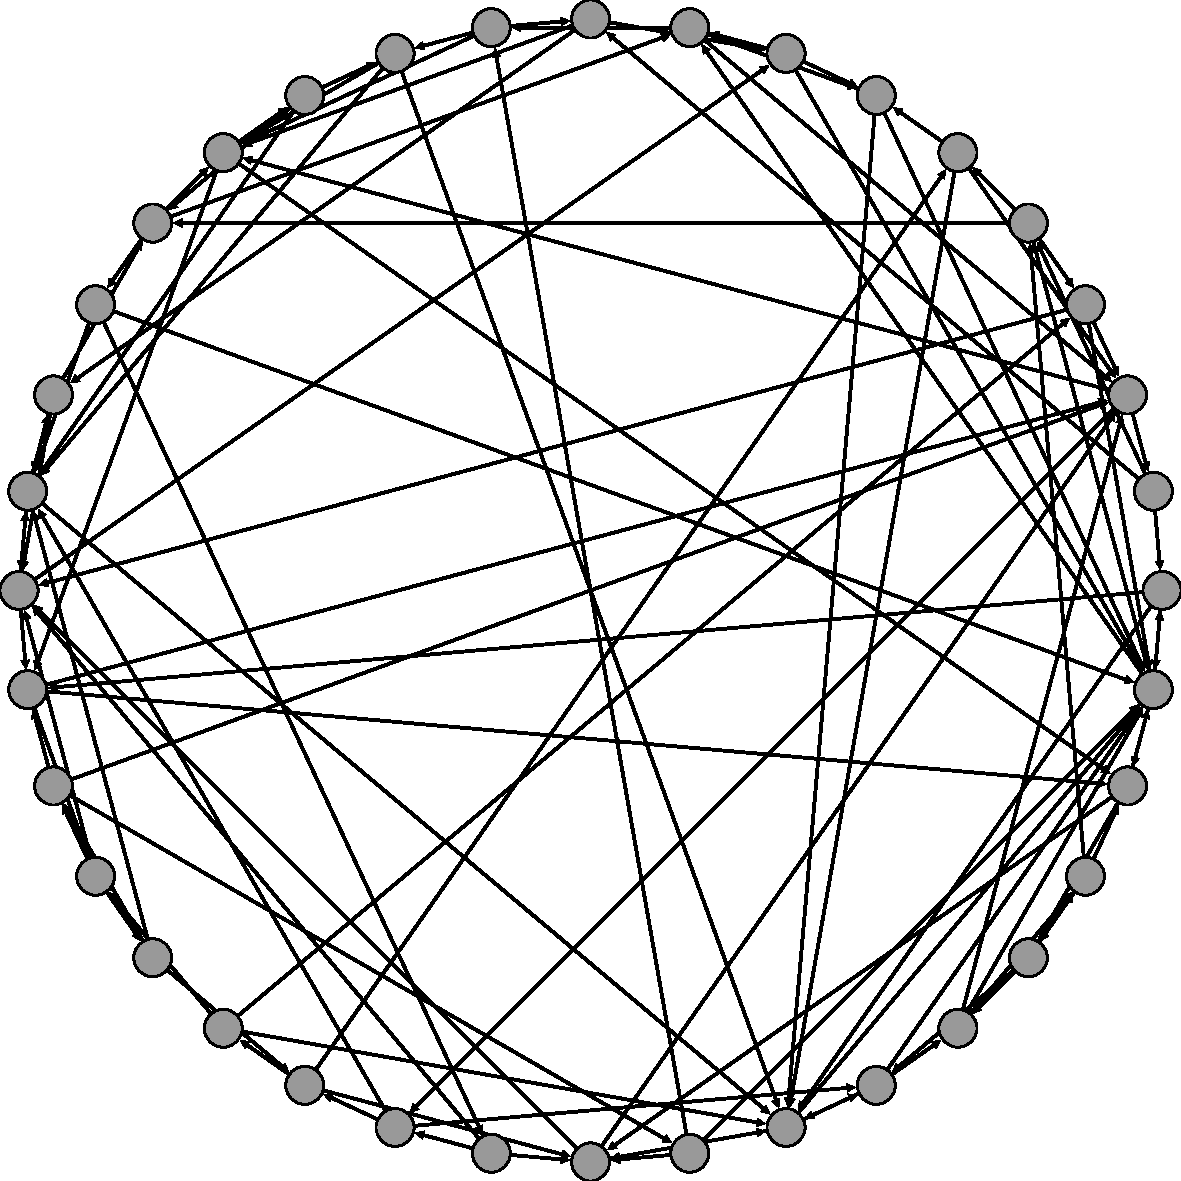
\includegraphics[width=\linewidth]{figures/hitratiobug}
    \caption{Visualization of publication message dissemination in
        PolderCast, which revealed a bug in the implementation of hit-ratio
        calculation}
   \label{fig:hitratiobug}
\end{figure}

When implementing hit-ratio calculation in the Collector, producing a
visualization of the publication message dissemination revealed a bug in the implementation code.
In PolderCast, the hit-ratio in the absence of churn should be 100\%.
However, the Collector would consistently calculate the hit-ratio to
97\%. Usually, the first step in debugging such issues is to isolate the
problem. In this case, there could be a software bug in the
implementation of the pub/sub protocol itself, or the bug might be in
the implementation of the hit-ratio calculation. Using \demo, we were
able to quickly isolate the problem. By producing a visualization of the
publication message dissemination, seen in Figure~\ref{fig:hitratiobug},
we were able to visually confirm that all nodes that took part in the dissemination
received the message. Furthermore, we could confirm this observation by
using the Statistics component in Gephi, which enables calculation of
the number of connected components in the graph.  The calculation
revealed that the graph is a single strongly connected component, i.e.\
from any node in the graph there is a directed path to any other node.
This means that every node received the publication.  However, the
Collector still calculated the hit-ratio to 97\%. This indicates that
the problem is not with the implementation of the protocol, but with the
implementation of the hit-ratio calculation. And indeed, by inspecting
the hit-ratio calculation in the Collector, we revealed a
\emph{off-by-one} software bug, leading to incorrect hit-ratio result.

Debugging is a major part of developing software, and arguably the most
time consuming. And debugging distributed systems is especially hard.
Any tool that aids in debugging is highly valuable to any developer. As
a tool for debugging, \demo{} can aid in both discovering and resolving
bugs, as it provides the developer with instant visual feedback of the
protocol behaviour.


\subsection{Using Test-Driven Development}

Software Development Methodology is an active area of research
which is in part driven by the business needs of the private
sector\cite{janzen2005test}. One popular practice is so-called Test-Driven
Development (TDD). The promoters of TDD claims it increases
productivity and reduces the number of bugs and defects in the
code significantly~\cite{beck2003test}. Research
efforts performed at IBM~\cite{maximilien2003assessing} seems to
lend credibility to these claims. However, the use of TDD is not
prevalent in academia, and in~\cite{janzen2005test} they
recommend further research into the field in order to better
determine its effects.

Using TDD means writing tests before writing any code. There are
different types of test. \emph{unit tests} targets small,
independent pieces of code, typically methods within a single
module or component, while \emph{integration tests} aim to test
code across such modules and components in order to determine
how well they integrate with each other. In our work, we only
took advantage of Unit Tests where suitable using the
JUnit~\cite{junit} and Mockito~\cite{mockito} libraries.
We could also have benefited from a suite of integration tests,
as our implementation is heavily dependent on interoperating
components, as well as file and network IO\@. However, writing
these sort of tests would simply be too time consuming compared
to writing smaller unit tests.

The TDD approach to software development is best described through the
Red-Green-Refactor mantra, which is a central part of the
TDD-philosophy. It can be described through the following steps:

\begin{description}
    \item[Step 1:] Write a test that fails. (Red)
    \item[Step 2:] Make the test pass. (Green)
    \item[Step 3:] Refactor the code while making sure the test
        still passes. (Refactor)
\end{description}

In our experience this routine has been helpful when working
with our implementation code, as it enables us as developer to
refactor with confidence achieving more maintainable code and a
more thoughtful software design. Since we share our
implementation code with the research community by hosting it in
a open repository, any tool or method that helps us improve the
design and maintainability of our project is of great value to
us. Using TDD forced us to think more deeply about what
functionality to implement and how to structure and split the
problem domain into smaller function points. We believe that in
the end, following TDD where its suitable is beneficial to both
programmer productivity as well as programmer happiness. Also,
we are confident that this practice decreased the amount of
technical debt in our project, a problem we find to be commonplace in academia.

\subsection{Sharing Code with the Community}

We believe sharing our code is to the benefit of both \demo{} and the
community. During our presentation at DEBS 2014, the interest in our
tool was high, and we received a fair amount of requests for our
implementation code. Sharing our code by hosting it publicly will
hopefully allow the tool to grow from a prototype into mature product by
allowing anyone to contribute with improvements and bug fixes. It is our
hope that \demo{} will be a lasting contribution to the research
community, and hosting the code publicly is a key part in ensuring the
future of the tool.

\section{Chapter Summary}


\chapter{Testing and Evaluation}
% This chapter should include expanding the experiments done in
% poldercast paper using peernet implementations of poldercast and using
% vizpub as a tool for evaluating the experiments in order to test it as
% a tool. Emphasis should be
% put on what metrics are evaluated which is not included in the
% original poldercast paper.
\label{ch:evaluation}
In this chapter, we utilize \demo{} in order to extend the evaluation of
PolderCast and Scribe found in~\cite{Setty:2012} on a set of topology
metrics. These metrics are afforded to us for ``free'' by the Gephi
framework through the Statistics API included in the \emph{Gephi
    Toolkit}.

\section{Experimental Setup}

We run PolderCast and Scribe in PeerNet using the simulation mode. The
Simulations consists of 1000 PeerNet cycles as well as 1000 reporter
intervals. We use workloads both from Facebook~\cite{} and
Twitter~\cite{} in order to model subscriptions. As mentioned in
Chapter~\ref{ch:vizpub}, the Facebook data trace include 3 million user
profiles along with 28.3 million friend relations. The Twitter dataset
consists of 41.7 million distinct users and 1.47 billion
follow/followed relations.

The social relations in Facebook are reciprocal, which leads us to model
bidirectional subscriptions. More specifically, a Facebook user is
modeled as a topic. The friends list of the particular user profile
constitutes its subscription list. All of the entries in this list will
include the original user in their own lists of subscriptions.
Relationships in Twitter however, are unidirectional. When using the
Twitter trace, users are also modeled as topics, but here the list of
subscriptions are formed on the basis of the ``following'' list of the
particular  user profile. The entries in this list are not required to
follow back, therefore subscriptions are also unidirectional.

Churn is based on the Skype super-peer trace from~\cite{}, tracing 4000
nodes for 4 weeks, tracking their joining and leaving timestamps. We
scale churn to include the first day of this trace in order to not
introduce a churn rate which is unrealistically high. For latency
between node pairs, we use the King dataset found in~cite{}.

\section{Experimental Restrictions}

\section{Results}

\begin{figure}
    \centering
    % GNUPLOT: LaTeX picture with Postscript
\begingroup
  \makeatletter
  \providecommand\color[2][]{%
    \GenericError{(gnuplot) \space\space\space\@spaces}{%
      Package color not loaded in conjunction with
      terminal option `colourtext'%
    }{See the gnuplot documentation for explanation.%
    }{Either use 'blacktext' in gnuplot or load the package
      color.sty in LaTeX.}%
    \renewcommand\color[2][]{}%
  }%
  \providecommand\includegraphics[2][]{%
    \GenericError{(gnuplot) \space\space\space\@spaces}{%
      Package graphicx or graphics not loaded%
    }{See the gnuplot documentation for explanation.%
    }{The gnuplot epslatex terminal needs graphicx.sty or graphics.sty.}%
    \renewcommand\includegraphics[2][]{}%
  }%
  \providecommand\rotatebox[2]{#2}%
  \@ifundefined{ifGPcolor}{%
    \newif\ifGPcolor
    \GPcolortrue
  }{}%
  \@ifundefined{ifGPblacktext}{%
    \newif\ifGPblacktext
    \GPblacktexttrue
  }{}%
  % define a \g@addto@macro without @ in the name:
  \let\gplgaddtomacro\g@addto@macro
  % define empty templates for all commands taking text:
  \gdef\gplbacktext{}%
  \gdef\gplfronttext{}%
  \makeatother
  \ifGPblacktext
    % no textcolor at all
    \def\colorrgb#1{}%
    \def\colorgray#1{}%
  \else
    % gray or color?
    \ifGPcolor
      \def\colorrgb#1{\color[rgb]{#1}}%
      \def\colorgray#1{\color[gray]{#1}}%
      \expandafter\def\csname LTw\endcsname{\color{white}}%
      \expandafter\def\csname LTb\endcsname{\color{black}}%
      \expandafter\def\csname LTa\endcsname{\color{black}}%
      \expandafter\def\csname LT0\endcsname{\color[rgb]{1,0,0}}%
      \expandafter\def\csname LT1\endcsname{\color[rgb]{0,1,0}}%
      \expandafter\def\csname LT2\endcsname{\color[rgb]{0,0,1}}%
      \expandafter\def\csname LT3\endcsname{\color[rgb]{1,0,1}}%
      \expandafter\def\csname LT4\endcsname{\color[rgb]{0,1,1}}%
      \expandafter\def\csname LT5\endcsname{\color[rgb]{1,1,0}}%
      \expandafter\def\csname LT6\endcsname{\color[rgb]{0,0,0}}%
      \expandafter\def\csname LT7\endcsname{\color[rgb]{1,0.3,0}}%
      \expandafter\def\csname LT8\endcsname{\color[rgb]{0.5,0.5,0.5}}%
    \else
      % gray
      \def\colorrgb#1{\color{black}}%
      \def\colorgray#1{\color[gray]{#1}}%
      \expandafter\def\csname LTw\endcsname{\color{white}}%
      \expandafter\def\csname LTb\endcsname{\color{black}}%
      \expandafter\def\csname LTa\endcsname{\color{black}}%
      \expandafter\def\csname LT0\endcsname{\color{black}}%
      \expandafter\def\csname LT1\endcsname{\color{black}}%
      \expandafter\def\csname LT2\endcsname{\color{black}}%
      \expandafter\def\csname LT3\endcsname{\color{black}}%
      \expandafter\def\csname LT4\endcsname{\color{black}}%
      \expandafter\def\csname LT5\endcsname{\color{black}}%
      \expandafter\def\csname LT6\endcsname{\color{black}}%
      \expandafter\def\csname LT7\endcsname{\color{black}}%
      \expandafter\def\csname LT8\endcsname{\color{black}}%
    \fi
  \fi
  \setlength{\unitlength}{0.0500bp}%
  \begin{picture}(7200.00,5040.00)%
    \gplgaddtomacro\gplbacktext{%
      \csname LTb\endcsname%
      \put(1342,704){\makebox(0,0)[r]{\strut{} 0.0001}}%
      \csname LTb\endcsname%
      \put(1342,1722){\makebox(0,0)[r]{\strut{} 0.001}}%
      \csname LTb\endcsname%
      \put(1342,2740){\makebox(0,0)[r]{\strut{} 0.01}}%
      \csname LTb\endcsname%
      \put(1342,3757){\makebox(0,0)[r]{\strut{} 0.1}}%
      \csname LTb\endcsname%
      \put(1342,4775){\makebox(0,0)[r]{\strut{} 1}}%
      \csname LTb\endcsname%
      \put(1474,484){\makebox(0,0){\strut{} 0}}%
      \csname LTb\endcsname%
      \put(1893,484){\makebox(0,0){\strut{} 100}}%
      \csname LTb\endcsname%
      \put(2311,484){\makebox(0,0){\strut{} 200}}%
      \csname LTb\endcsname%
      \put(2730,484){\makebox(0,0){\strut{} 300}}%
      \csname LTb\endcsname%
      \put(3148,484){\makebox(0,0){\strut{} 400}}%
      \csname LTb\endcsname%
      \put(3567,484){\makebox(0,0){\strut{} 500}}%
      \csname LTb\endcsname%
      \put(3985,484){\makebox(0,0){\strut{} 600}}%
      \csname LTb\endcsname%
      \put(4404,484){\makebox(0,0){\strut{} 700}}%
      \csname LTb\endcsname%
      \put(4822,484){\makebox(0,0){\strut{} 800}}%
      \csname LTb\endcsname%
      \put(5241,484){\makebox(0,0){\strut{} 900}}%
      \csname LTb\endcsname%
      \put(5659,484){\makebox(0,0){\strut{} 1000}}%
      \put(5791,704){\makebox(0,0)[l]{\strut{} 0}}%
      \put(5791,1111){\makebox(0,0)[l]{\strut{} 100}}%
      \put(5791,1518){\makebox(0,0)[l]{\strut{} 200}}%
      \put(5791,1925){\makebox(0,0)[l]{\strut{} 300}}%
      \put(5791,2332){\makebox(0,0)[l]{\strut{} 400}}%
      \put(5791,2740){\makebox(0,0)[l]{\strut{} 500}}%
      \put(5791,3147){\makebox(0,0)[l]{\strut{} 600}}%
      \put(5791,3554){\makebox(0,0)[l]{\strut{} 700}}%
      \put(5791,3961){\makebox(0,0)[l]{\strut{} 800}}%
      \put(5791,4368){\makebox(0,0)[l]{\strut{} 900}}%
      \put(5791,4775){\makebox(0,0)[l]{\strut{} 1000}}%
      \put(176,2739){\rotatebox{-270}{\makebox(0,0){\strut{}Avg. Clustering Coefficient}}}%
      \put(6692,2739){\rotatebox{-270}{\makebox(0,0){\strut{}Network Size}}}%
      \put(3566,154){\makebox(0,0){\strut{}Reporter Intervals}}%
    }%
    \gplgaddtomacro\gplfronttext{%
      \csname LTb\endcsname%
      \put(4672,1757){\makebox(0,0)[r]{\strut{}PolderCast (Facebook)}}%
      \csname LTb\endcsname%
      \put(4672,1537){\makebox(0,0)[r]{\strut{}PolderCast (Twitter)}}%
      \csname LTb\endcsname%
      \put(4672,1317){\makebox(0,0)[r]{\strut{}Scribe (Facebook)}}%
      \csname LTb\endcsname%
      \put(4672,1097){\makebox(0,0)[r]{\strut{}Scribe (Twitter)}}%
      \csname LTb\endcsname%
      \put(4672,877){\makebox(0,0)[r]{\strut{}Network Size}}%
    }%
    \gplbacktext
    \put(0,0){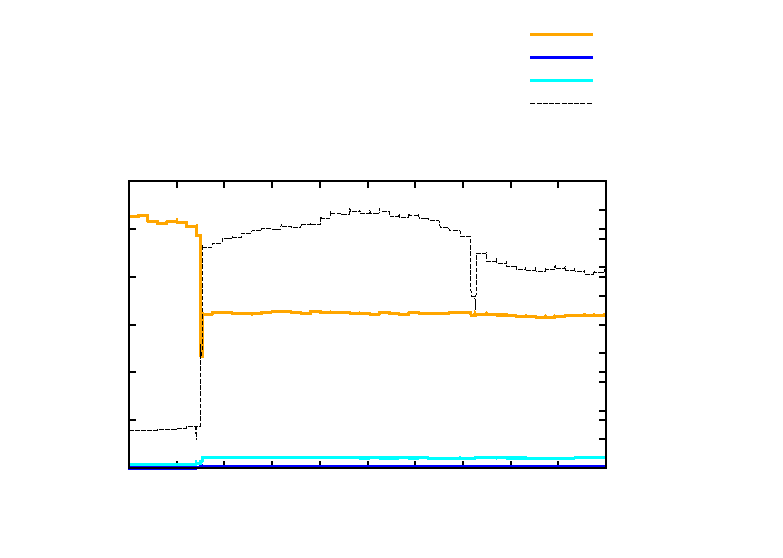
\includegraphics{eval_cc}}%
    \gplfronttext
  \end{picture}%
\endgroup

    \caption{Clustering Coefficient of PolderCast and Scribe}
    \label{fig:eval_cc}
\end{figure}

\begin{figure}
    \centering
    % GNUPLOT: LaTeX picture with Postscript
\begingroup
  \makeatletter
  \providecommand\color[2][]{%
    \GenericError{(gnuplot) \space\space\space\@spaces}{%
      Package color not loaded in conjunction with
      terminal option `colourtext'%
    }{See the gnuplot documentation for explanation.%
    }{Either use 'blacktext' in gnuplot or load the package
      color.sty in LaTeX.}%
    \renewcommand\color[2][]{}%
  }%
  \providecommand\includegraphics[2][]{%
    \GenericError{(gnuplot) \space\space\space\@spaces}{%
      Package graphicx or graphics not loaded%
    }{See the gnuplot documentation for explanation.%
    }{The gnuplot epslatex terminal needs graphicx.sty or graphics.sty.}%
    \renewcommand\includegraphics[2][]{}%
  }%
  \providecommand\rotatebox[2]{#2}%
  \@ifundefined{ifGPcolor}{%
    \newif\ifGPcolor
    \GPcolortrue
  }{}%
  \@ifundefined{ifGPblacktext}{%
    \newif\ifGPblacktext
    \GPblacktexttrue
  }{}%
  % define a \g@addto@macro without @ in the name:
  \let\gplgaddtomacro\g@addto@macro
  % define empty templates for all commands taking text:
  \gdef\gplbacktext{}%
  \gdef\gplfronttext{}%
  \makeatother
  \ifGPblacktext
    % no textcolor at all
    \def\colorrgb#1{}%
    \def\colorgray#1{}%
  \else
    % gray or color?
    \ifGPcolor
      \def\colorrgb#1{\color[rgb]{#1}}%
      \def\colorgray#1{\color[gray]{#1}}%
      \expandafter\def\csname LTw\endcsname{\color{white}}%
      \expandafter\def\csname LTb\endcsname{\color{black}}%
      \expandafter\def\csname LTa\endcsname{\color{black}}%
      \expandafter\def\csname LT0\endcsname{\color[rgb]{1,0,0}}%
      \expandafter\def\csname LT1\endcsname{\color[rgb]{0,1,0}}%
      \expandafter\def\csname LT2\endcsname{\color[rgb]{0,0,1}}%
      \expandafter\def\csname LT3\endcsname{\color[rgb]{1,0,1}}%
      \expandafter\def\csname LT4\endcsname{\color[rgb]{0,1,1}}%
      \expandafter\def\csname LT5\endcsname{\color[rgb]{1,1,0}}%
      \expandafter\def\csname LT6\endcsname{\color[rgb]{0,0,0}}%
      \expandafter\def\csname LT7\endcsname{\color[rgb]{1,0.3,0}}%
      \expandafter\def\csname LT8\endcsname{\color[rgb]{0.5,0.5,0.5}}%
    \else
      % gray
      \def\colorrgb#1{\color{black}}%
      \def\colorgray#1{\color[gray]{#1}}%
      \expandafter\def\csname LTw\endcsname{\color{white}}%
      \expandafter\def\csname LTb\endcsname{\color{black}}%
      \expandafter\def\csname LTa\endcsname{\color{black}}%
      \expandafter\def\csname LT0\endcsname{\color{black}}%
      \expandafter\def\csname LT1\endcsname{\color{black}}%
      \expandafter\def\csname LT2\endcsname{\color{black}}%
      \expandafter\def\csname LT3\endcsname{\color{black}}%
      \expandafter\def\csname LT4\endcsname{\color{black}}%
      \expandafter\def\csname LT5\endcsname{\color{black}}%
      \expandafter\def\csname LT6\endcsname{\color{black}}%
      \expandafter\def\csname LT7\endcsname{\color{black}}%
      \expandafter\def\csname LT8\endcsname{\color{black}}%
    \fi
  \fi
  \setlength{\unitlength}{0.0500bp}%
  \begin{picture}(7200.00,5040.00)%
    \gplgaddtomacro\gplbacktext{%
      \csname LTb\endcsname%
      \put(1078,704){\makebox(0,0)[r]{\strut{} 0}}%
      \put(1078,1163){\makebox(0,0)[r]{\strut{} 1000}}%
      \put(1078,1621){\makebox(0,0)[r]{\strut{} 2000}}%
      \put(1078,2080){\makebox(0,0)[r]{\strut{} 3000}}%
      \put(1078,2538){\makebox(0,0)[r]{\strut{} 4000}}%
      \put(1078,2997){\makebox(0,0)[r]{\strut{} 5000}}%
      \put(1078,3455){\makebox(0,0)[r]{\strut{} 6000}}%
      \put(1210,484){\makebox(0,0){\strut{} 0}}%
      \put(1655,484){\makebox(0,0){\strut{} 100}}%
      \put(2100,484){\makebox(0,0){\strut{} 200}}%
      \put(2545,484){\makebox(0,0){\strut{} 300}}%
      \put(2990,484){\makebox(0,0){\strut{} 400}}%
      \put(3435,484){\makebox(0,0){\strut{} 500}}%
      \put(3879,484){\makebox(0,0){\strut{} 600}}%
      \put(4324,484){\makebox(0,0){\strut{} 700}}%
      \put(4769,484){\makebox(0,0){\strut{} 800}}%
      \put(5214,484){\makebox(0,0){\strut{} 900}}%
      \put(5659,484){\makebox(0,0){\strut{} 1000}}%
      \put(5791,704){\makebox(0,0)[l]{\strut{} 0}}%
      \put(5791,979){\makebox(0,0)[l]{\strut{} 100}}%
      \put(5791,1254){\makebox(0,0)[l]{\strut{} 200}}%
      \put(5791,1529){\makebox(0,0)[l]{\strut{} 300}}%
      \put(5791,1804){\makebox(0,0)[l]{\strut{} 400}}%
      \put(5791,2080){\makebox(0,0)[l]{\strut{} 500}}%
      \put(5791,2355){\makebox(0,0)[l]{\strut{} 600}}%
      \put(5791,2630){\makebox(0,0)[l]{\strut{} 700}}%
      \put(5791,2905){\makebox(0,0)[l]{\strut{} 800}}%
      \put(5791,3180){\makebox(0,0)[l]{\strut{} 900}}%
      \put(5791,3455){\makebox(0,0)[l]{\strut{} 1000}}%
      \put(176,2079){\rotatebox{-270}{\makebox(0,0){\strut{}Betweenness Centrality}}}%
      \put(6692,2079){\rotatebox{-270}{\makebox(0,0){\strut{}Network Size}}}%
      \put(3434,154){\makebox(0,0){\strut{}Reporter Intervals}}%
    }%
    \gplgaddtomacro\gplfronttext{%
      \csname LTb\endcsname%
      \put(4804,4867){\makebox(0,0)[r]{\strut{}PolderCast (Facebook)}}%
      \csname LTb\endcsname%
      \put(4804,4647){\makebox(0,0)[r]{\strut{}PolderCast (Twitter)}}%
      \csname LTb\endcsname%
      \put(4804,4427){\makebox(0,0)[r]{\strut{}Scribe (Facebook)}}%
      \csname LTb\endcsname%
      \put(4804,4207){\makebox(0,0)[r]{\strut{}Scribe (Twitter)}}%
      \csname LTb\endcsname%
      \put(4804,3987){\makebox(0,0)[r]{\strut{}Network Size}}%
    }%
    \gplbacktext
    \put(0,0){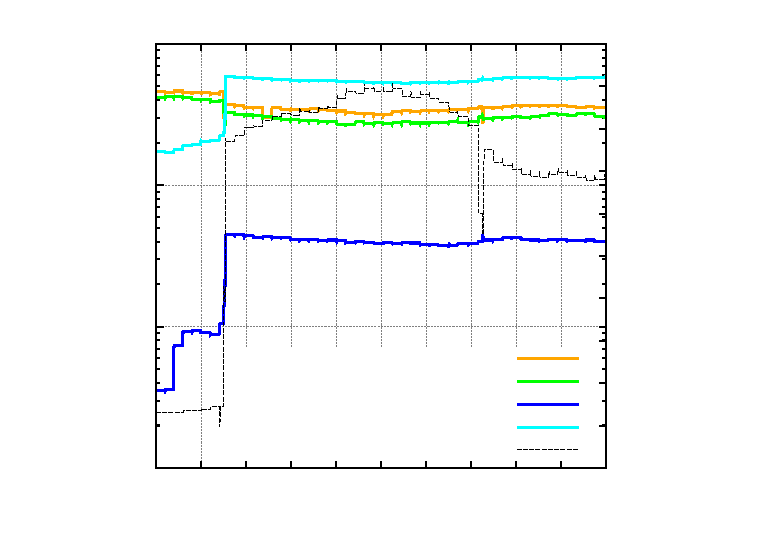
\includegraphics{eval_betweenness}}%
    \gplfronttext
  \end{picture}%
\endgroup

    \caption{Betweenness centrality of PolderCast and Scribe}
    \label{fig:eval_betweenness}
\end{figure}


\chapter{Conclusion and Future Work}
% What have we shown? We propose a tool for visualizing metrics, we
% demonstrate its usefulness, we use this tool to evaluate two pub/sub
% systems, expanding the evaluation done in the poldercast paper. Then
% this chapter should include future work, implementing plugins etc.

%Drawbacks of vizpub:
% adds overhead
% file sizes does not scale well
\label{ch:conclusion-and-future-work}
\section{Conclusion}

\section{Future Work}

We believe there is a lot of potential for a tool such as \demo{}. What
we present in this thesis is currently only a prototype, but hopefully
it can serve as a starting point for further improvements. In this
section we will discuss some of these potential improvements to \demo{},
as well as some of the issues and limitations we faced in our implementation work.

\subsection{Resolve Hit-ratio Bug}

\subsection{Evaluate Topic Diameter}

\subsection{Improving Report File Sizes}

Currently, the biggest issue with \demo{} is scalability in terms of
file sizes. Both the Reporter and Collector stores temporary files
which can be quite large depending on the scale of the system in terms
of number of nodes, edges as well as number of topics and publication
messages being posted on each topic. During our experiments we ran into
several issues due to restrictions in disk quota on the machine cluster.
In particular, a high number of edges cause issues, especially if any
attributes are applied to them. But also the number of publication
messages will bloat file sizes of the temporary logs considerably. This
causes performance issues when the Collector collates these files into
the final report. The final report also scales poorly in terms of file
size due to the \gexf{} format being based on XML, which stores data in
a declarative text based format. The file sizes of the final report can
grow up to several gigabytes, which causes big performance issues when
opening these files in Gephi. Due to these performance issues we had to
restrict the scale of our experiments. This is unfortunate, and the
issues with performance should be addressed quickly in order to increase
the scalability of the system. Fortunately, there is a lot of
low-hanging fruit in terms of increasing the performance of the system,
as it is still in the prototype stage.

\subsection{Implementing Database Support}

\subsection{Gephi Performance Issues}

There are also performance issues with Gephi, as it is still in version
0.8.7. Currently, Gephi is very memory intensive, due to the data model
it uses for storing graphs. However, the authors have dealt with this
issue in the current development version, where the memory usage has
been significantly decreased. However, this version also breaks some
features which prevents us from using it. Another important point to
make regarding performance in Gephi is the use of OpenGL when rendering
graphs. This means that in order to open large graphs in Gephi, it is
necessary to use a computer with a dedicated graphics card. The bigger
the Graph, the more graphics capability is needed.

\subsection{Reporter Performance Issues}

The reporter has some performance issues due to allocating new Java
objects each time the Collector pulls data. This causes the Java process to
hang, as the garbage collector kicks in to clean up the heap. This is an
issue which should be fixed by allocating memory statically and
overwriting rather re-allocating. Also, this is a potential bottleneck
in the system with regards to memory usage. If the reports are very large, the Java
objects might occupy too much  memory, causing the Java process to
fail. However, this should only be an issue when  running simulations at
scale, where a process might include several simulated PeerNet nodes but only one
reporter.

\subsection{Visualizing with Custom Colors and Sizes}

Most of the visualizations in this thesis use text labels and color in
order to convey information regarding the performance of the pub/sub
system in question. However, it would also be interesting to visualize
metrics using shapes, sizes and custom colors. For example, edges could
be of different thickness, according to how many topic attributes were
added to them. Also, special nodes such as the \emph{rendezvous} nodes
in Scribe could have a custom color to them in order to identify them
easily. Alternatively, the nodes could be of a different sizes than
``regular'' nodes. This is different than the current way of applying
colors through the \emph{Statistics Component} in Gephi, as it is
dependent on the existence of a node attribute. Any custom color or size
would have to be applied by the Collector. However, due to a bug in the
software library used to build the \gexf{} files, this was not possible
to implement.


\subsection{Collector Scalability}

In the current implementation of \demo{}, the collector is run in a
single JVM instance, where the pub/sub nodes connect to it via TCP.\
There might be issues with the scalability in terms of number of
connections, as we have not been able to test the system with more than
30 connections. The Collector also serve as a single point of failure.
Ideally, the Collector should itself be a distributed system, with
built-in fault tolerance and a replication scheme. This is an important
if \demo{} is ever to be considered \emph{production ready}, i.e.\ ever
being used in real, deployed pub/sub systems. This is not a pressing
concern however, as \demo{} is still a far way from being production
ready, but hopefully it will be in the future.

\subsection{Including Associative Arrays in Gephi}

It would be useful to be able to store a map data structure on each
graph, i.e.\ associative arrays. If associative arrays were supported,
a user could derive information such as how many duplicate messages a
particular node received on a specific topic or single dissemination
session. Also, it would enable the user to see how many publication messages a
particular node sent or received for a specific topic. Implementing such
a structure will most likely involve modifying the source code of Gephi.
This is fully possible, since Gephi is an open source product and hosted
in a public repository.\footnote{\url{http://github.com/gephi/gephi}}
This would require quite an effort however, as the code base is quite
large and it would take time to gain the necessary insight into it.

\subsection{Implementing Global Attribute Visualization}

Currently, it is not possible to visualize graph attributes in Gephi, or
indeed list any global attribute in the graph. This would be a useful
feature to implement as a plugin. For example, it would be helpful to be
able to list all topics on the graph and sort then according to number
of subscribers. Our workaround for this is to apply a node label to all
nodes which describes a global attribute. Such global attributes include
hit-ratio and average control messages sent and received. Visualizing
these attributes on every node can be misleading, as it gives the
impression that the values are unique to every node. It would be better
to display these values in a separate panel, or perhaps even as a large
floating text label in the Graph view.

\subsection{\demo{} as an Interactive Monitoring System}

As mentioned, the visualization of pub/sub systems are done offline,
after the execution of the pub/sub system is finished. It is not
intended to be a real-time system, where data is pulled and metrics are
calculated during system execution. When inspecting the overlay using
the \emph{Visualization Unit}, users may delete nodes in order to
determine the effect it has on the overlay topology by recalculation
such metrics using the \emph{Statistics Component} in Gephi. However, it will
not affect any custom metrics which are calculated by the Collector such
as control messages sent and received as these metrics are calculated
after the execution of the pub/sub system. In order to affect such
metrics, the architecture would have to be changed in order to
accommodate for a two-way communication, where the Collector would be
able to issue commands to the pub/sub nodes. Also, the Collector would
have to collect data, calculate metrics and stream this information to
Gephi in real-time. Gephi does indeed include an API for streaming data,
so it is possible in theory, although in practice there are some issues
with this API.\ This would be incredibly useful however, both as a
monitoring system and as an environment for experimenting with protocols
and their behavior. For example, imagine being able to right-click a
node in Gephi, and ask this node leave the network. The Collector would
then issue a leave command to the node in question, and the user could
then potentially observe what happens in the Visualization Unit. The
interactivity of such a feature would be incredibly engaging and useful
both for developers and researchers, as well as students. Such
a feature requires extensive re-engineering of \demo{}, but would be
well worth the effort.

\subsection{Playback issues in the Timeline component}

We encountered some issues related to the playback of dynamic
graphs in Gephi. The playback is based on time intervals, where the
start and end bounds for the interval is encoded as a double. As you
play back the graph evolution, these bounds suffer from rounding errors,
which might lead to an interval that overlaps to simulation states.
These intervals are effectively filter, stripping the graph of nodes and
edges that do not belong in the defined interval. However, if the
interval crosses the boundary of two different simulation states, the
edges and nodes from both states will be included, which often leads to
a sudden increase in number of edges during the animation, which
abruptly disappear again. However, this issue is easily worked around by
defining a sufficiently short interval. We usually set the interval
bound to be of length 0.1, as this in our experience never leads to the
issues with the time interval overlapping different states. We confirmed
this by playing back the graph and controlling the start and end bounds
output on the Filter component, as well as visually confirming the
absence of any edge animation irregularities. Testing with the Cyclon
protocol, we were also able to visually confirm that the number of edges
remain consistent for each cycle in the context pane on the top right
side of the Gephi GUI\@.


\backmatter{}
\printbibliography{}
\end{document}
